\documentclass[8pt,aspectratio=169]{beamer}
\usetheme{Madrid}
\usepackage{graphicx,booktabs,adjustbox,multicol,amsmath,amssymb,listings,xcolor,colortbl}
\definecolor{mlblue}{RGB}{0,102,204}
\definecolor{mlpurple}{RGB}{51,51,178}
\definecolor{mllavender}{RGB}{173,173,224}
\definecolor{mllavender2}{RGB}{193,193,232}
\definecolor{mllavender3}{RGB}{204,204,235}
\definecolor{mllavender4}{RGB}{214,214,239}
\definecolor{mlorange}{RGB}{255,127,14}
\definecolor{mlgreen}{RGB}{44,160,44}
\definecolor{mlred}{RGB}{214,39,40}
\definecolor{mlgray}{RGB}{127,127,127}
% Solidity colors
\definecolor{solkeyword}{RGB}{0,102,153}
\definecolor{solstring}{RGB}{163,21,21}
\definecolor{solcomment}{RGB}{0,128,0}
\definecolor{solnumber}{RGB}{0,128,128}
\setbeamercolor{palette primary}{bg=mllavender3,fg=mlpurple}
\setbeamercolor{palette secondary}{bg=mllavender2,fg=mlpurple}
\setbeamercolor{palette tertiary}{bg=mllavender,fg=white}
\setbeamercolor{palette quaternary}{bg=mlpurple,fg=white}
\setbeamercolor{structure}{fg=mlpurple}
\setbeamercolor{title}{fg=mlpurple}
\setbeamercolor{frametitle}{fg=mlpurple,bg=mllavender3}
\setbeamercolor{block title}{bg=mllavender2,fg=mlpurple}
\setbeamercolor{block body}{bg=mllavender4,fg=black}
\setbeamertemplate{navigation symbols}{}
\setbeamertemplate{itemize items}[circle]
\setbeamersize{text margin left=5mm,text margin right=5mm}
\newcommand{\bottomnote}[1]{\vfill\vspace{-2mm}\textcolor{mllavender2}{\rule{\textwidth}{0.4pt}}\vspace{1mm}\footnotesize\textbf{#1}}
% Solidity language definition
\lstdefinelanguage{Solidity}{
  keywords={pragma, solidity, contract, function, public, private, external, internal, view, pure, payable, returns, return, if, else, for, while, mapping, address, uint, uint256, int, string, bool, bytes, bytes32, event, emit, modifier, require, constructor, memory, storage, calldata, msg, sender, value, this, new, delete, true, false, import, is, constant, override, virtual, interface, library, abstract, struct, enum, unchecked, assembly, abi, encode, decode, keccak256, receive, fallback},
  keywordstyle=\color{solkeyword}\bfseries,
  sensitive=true,
  comment=[l]{//},
  morecomment=[s]{/*}{*/},
  commentstyle=\color{solcomment}\ttfamily,
  stringstyle=\color{solstring}\ttfamily,
  morestring=[b]',
  morestring=[b]"
}
\lstset{language=Solidity,basicstyle=\ttfamily\scriptsize,breaklines=true,frame=single,backgroundcolor=\color{mllavender4},numbers=left,numberstyle=\tiny\color{mlgray},numbersep=5pt,tabsize=2,showstringspaces=false}
\usepackage{tikz,pgfplots}
\pgfplotsset{compat=1.18}
\usetikzlibrary{arrows.meta,positioning,shapes.geometric,calc,chains,decorations.pathmorphing,automata,fit}
\title{Real-World Assets \& Tokenization: Bridging TradFi and DeFi}
\subtitle{Standalone Technical Lecture}
\author{Prof.~Dr.~Joerg Osterrieder}
\institute{University Lecture Series}
\date{\today}

\begin{document}

%% ============================================================
%% OPENING FRAMES
%% ============================================================

% Frame 1: Title
\begin{frame}
\titlepage
\end{frame}

% Frame 2: Lecture Roadmap
\begin{frame}{Lecture Roadmap}
\begin{columns}[T]
\column{0.55\textwidth}
\vspace{2mm}
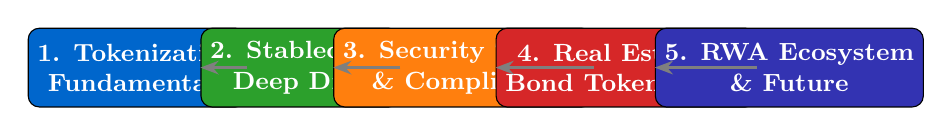
\begin{tikzpicture}[scale=0.9]
  \node[draw,fill=mlblue,text=white,rounded corners=4pt,
        minimum width=2.0cm,minimum height=1.0cm,align=center,font=\small\bfseries]
        (b1) at (0,0) {1. Tokenization\\Fundamentals};
  \node[draw,fill=mlgreen,text=white,rounded corners=4pt,
        minimum width=2.0cm,minimum height=1.0cm,align=center,font=\small\bfseries]
        (b2) at (2.3,0) {2. Stablecoins\\Deep Dive};
  \node[draw,fill=mlorange,text=white,rounded corners=4pt,
        minimum width=2.0cm,minimum height=1.0cm,align=center,font=\small\bfseries]
        (b3) at (4.6,0) {3. Security Tokens\\\& Compliance};
  \node[draw,fill=mlred,text=white,rounded corners=4pt,
        minimum width=2.0cm,minimum height=1.0cm,align=center,font=\small\bfseries]
        (b4) at (6.9,0) {4. Real Estate \&\\Bond Tokenization};
  \node[draw,fill=mlpurple,text=white,rounded corners=4pt,
        minimum width=2.0cm,minimum height=1.0cm,align=center,font=\small\bfseries]
        (b5) at (9.2,0) {5. RWA Ecosystem\\\& Future};
  \draw[-{Stealth},thick,mlgray] (b1.east) -- (b2.west);
  \draw[-{Stealth},thick,mlgray] (b2.east) -- (b3.west);
  \draw[-{Stealth},thick,mlgray] (b3.east) -- (b4.west);
  \draw[-{Stealth},thick,mlgray] (b4.east) -- (b5.west);
\end{tikzpicture}
\vspace{3mm}

\column{0.45\textwidth}
\begin{block}{Learning Objectives}
\footnotesize
\begin{itemize}
  \item Understand tokenization mechanics and real-world asset classes
  \item Analyse stablecoin designs: fiat-backed, crypto-backed, algorithmic
  \item Evaluate security token standards and compliance frameworks
  \item Assess real estate and bond tokenization case studies
  \item Survey the RWA ecosystem, institutional adoption, and future outlook
\end{itemize}
\end{block}
\vspace{1mm}
\begin{block}{Prerequisites}
\footnotesize
\begin{itemize}
  \item Lessons 1--5: Blockchain fundamentals, smart contracts, DeFi
  \item Basic familiarity with traditional finance (bonds, real estate, securities)
\end{itemize}
\end{block}
\end{columns}
\bottomnote{Duration: 90 minutes | 5 sections | \textasciitilde55 frames | Prerequisite: Lessons 1--5}
\end{frame}

% Frame 3: Table of Contents
\begin{frame}{Table of Contents}
\tableofcontents
\bottomnote{Navigate through 5 sections from tokenization fundamentals to the future of the RWA ecosystem}
\end{frame}

%% ============================================================
%% SECTION 1: TOKENIZATION FUNDAMENTALS
%% ============================================================
\section{Tokenization Fundamentals}

% Frame 4: Section 1 Divider
\begin{frame}{}
\begin{beamercolorbox}[sep=12pt,center,rounded=true,shadow=true]{palette quaternary}
  {\Large\bfseries Section 1: Tokenization Fundamentals}\\[6pt]
  {\normalsize What is tokenization, asset classes, token standards, and the fractionalization revolution}
\end{beamercolorbox}
\vspace{4mm}
\begin{columns}[T]
\column{0.5\textwidth}
\begin{block}{What You Will Learn}
\footnotesize
\begin{itemize}
  \item What tokenization means and how it digitizes ownership
  \item Tokenizable asset classes: real estate, bonds, commodities, art
  \item Token standards: ERC-20, ERC-721, ERC-1155, ERC-3643
  \item Benefits: fractional ownership, 24/7 markets, global access
\end{itemize}
\end{block}
\column{0.5\textwidth}
\begin{block}{Frames in This Section}
\footnotesize
\begin{itemize}
  \item Frame 5: What is Tokenization?
  \item Frame 6: Tokenizable Asset Classes
  \item Frame 7: Token Standards for RWA
  \item Frame 8: ERC-20 Asset Token Contract (Code)
  \item Frame 9: Fractionalization Mechanics
  \item Frame 10: Benefits of Tokenization
  \item Frame 11: Challenges of Tokenization
  \item Frame 12: The Oracle Problem for RWA
  \item Frame 13: Tokenization Market Map
  \item Frame 14: Section 1 Summary
\end{itemize}
\end{block}
\end{columns}
\bottomnote{Section 1 of 5 | Frames 4--14}
\end{frame}

% Frame 5: What is Tokenization?
\begin{frame}{What is Tokenization?}
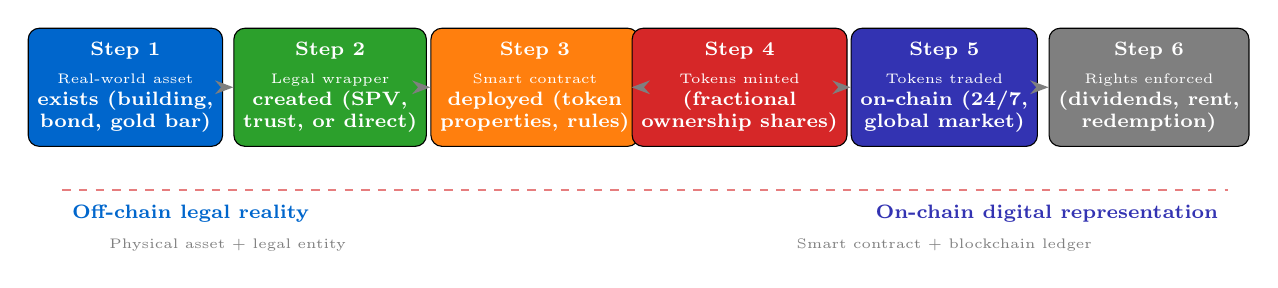
\begin{tikzpicture}[
  rwastep/.style={draw,rounded corners=4pt,minimum width=2.1cm,minimum height=1.5cm,
    align=center,font=\scriptsize\bfseries,text=white},
  rwaarrow/.style={-{Stealth},thick,mlgray}
]
  % Step nodes
  \node[rwastep,fill=mlblue] (s1) at (0,0) {Step 1\\[2pt]\normalfont\tiny Real-world asset\\exists (building,\\bond, gold bar)};
  \node[rwastep,fill=mlgreen] (s2) at (2.6,0) {Step 2\\[2pt]\normalfont\tiny Legal wrapper\\created (SPV,\\trust, or direct)};
  \node[rwastep,fill=mlorange] (s3) at (5.2,0) {Step 3\\[2pt]\normalfont\tiny Smart contract\\deployed (token\\properties, rules)};
  \node[rwastep,fill=mlred] (s4) at (7.8,0) {Step 4\\[2pt]\normalfont\tiny Tokens minted\\(fractional\\ownership shares)};
  \node[rwastep,fill=mlpurple] (s5) at (10.4,0) {Step 5\\[2pt]\normalfont\tiny Tokens traded\\on-chain (24/7,\\global market)};
  \node[rwastep,fill=mlgray] (s6) at (13.0,0) {Step 6\\[2pt]\normalfont\tiny Rights enforced\\(dividends, rent,\\redemption)};
  % Arrows
  \draw[rwaarrow] (s1.east) -- (s2.west);
  \draw[rwaarrow] (s2.east) -- (s3.west);
  \draw[rwaarrow] (s3.east) -- (s4.west);
  \draw[rwaarrow] (s4.east) -- (s5.west);
  \draw[rwaarrow] (s5.east) -- (s6.west);
  % Dashed separation line
  \draw[dashed,thick,mlred!60] (-0.8,-1.3) -- (14.0,-1.3);
  \node[font=\scriptsize,mlblue,anchor=west] at (-0.8,-1.6) {\textbf{Off-chain legal reality}};
  \node[font=\scriptsize,mlpurple,anchor=east] at (14.0,-1.6) {\textbf{On-chain digital representation}};
  % Labels below the line
  \node[font=\tiny,mlgray,anchor=north] at (1.3,-1.8) {Physical asset + legal entity};
  \node[font=\tiny,mlgray,anchor=north] at (10.4,-1.8) {Smart contract + blockchain ledger};
\end{tikzpicture}
\bottomnote{Tokenization creates a digital twin of asset ownership -- the legal wrapper ensures the token conveys real legal rights}
\end{frame}

% Frame 6: Tokenizable Asset Classes
\begin{frame}{Tokenizable Asset Classes}
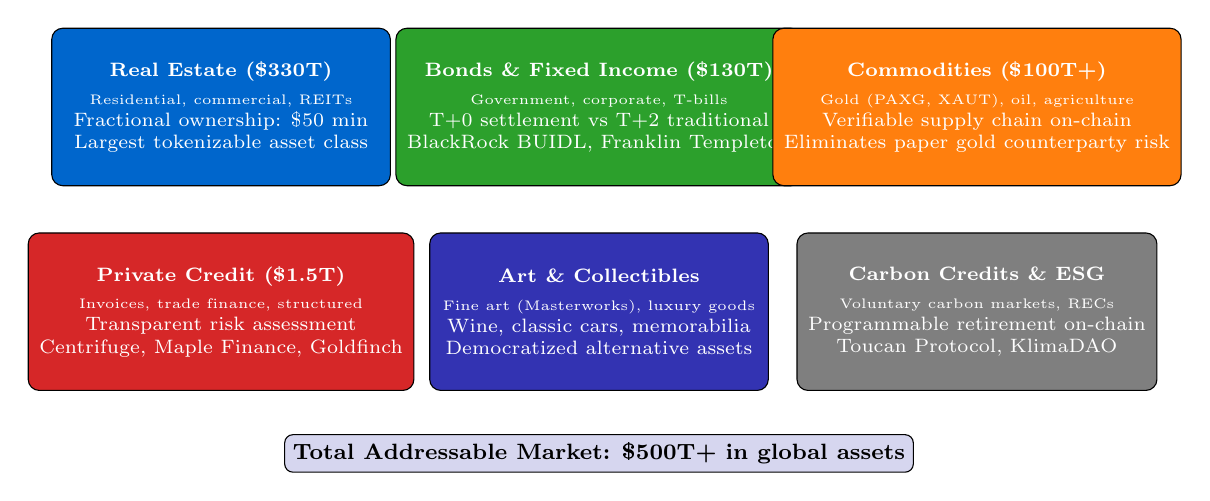
\begin{tikzpicture}[
  rwabox/.style={draw,rounded corners=4pt,minimum width=4.3cm,minimum height=2.0cm,
    align=center,font=\scriptsize,text=white,inner sep=4pt}
]
  % Row 1
  \node[rwabox,fill=mlblue] (a1) at (0,0) {\textbf{Real Estate (\$330T)}\\[2pt]
    \tiny Residential, commercial, REITs\\Fractional ownership: \$50 min\\Largest tokenizable asset class};
  \node[rwabox,fill=mlgreen] (a2) at (4.8,0) {\textbf{Bonds \& Fixed Income (\$130T)}\\[2pt]
    \tiny Government, corporate, T-bills\\T+0 settlement vs T+2 traditional\\BlackRock BUIDL, Franklin Templeton};
  \node[rwabox,fill=mlorange] (a3) at (9.6,0) {\textbf{Commodities (\$100T+)}\\[2pt]
    \tiny Gold (PAXG, XAUT), oil, agriculture\\Verifiable supply chain on-chain\\Eliminates paper gold counterparty risk};
  % Row 2
  \node[rwabox,fill=mlred] (a4) at (0,-2.6) {\textbf{Private Credit (\$1.5T)}\\[2pt]
    \tiny Invoices, trade finance, structured\\Transparent risk assessment\\Centrifuge, Maple Finance, Goldfinch};
  \node[rwabox,fill=mlpurple] (a5) at (4.8,-2.6) {\textbf{Art \& Collectibles}\\[2pt]
    \tiny Fine art (Masterworks), luxury goods\\Wine, classic cars, memorabilia\\Democratized alternative assets};
  \node[rwabox,fill=mlgray] (a6) at (9.6,-2.6) {\textbf{Carbon Credits \& ESG}\\[2pt]
    \tiny Voluntary carbon markets, RECs\\Programmable retirement on-chain\\Toucan Protocol, KlimaDAO};
  % Total addressable market
  \node[draw,fill=mllavender4,rounded corners=3pt,font=\footnotesize\bfseries,inner sep=3pt]
    at (4.8,-4.4) {Total Addressable Market: \$500T+ in global assets};
\end{tikzpicture}
\bottomnote{Even tokenizing 1\% of global real estate (\$330T) would create a \$3.3T on-chain market -- larger than all of DeFi today}
\end{frame}

% Frame 7: Token Standards for RWA
\begin{frame}{Token Standards for RWA}
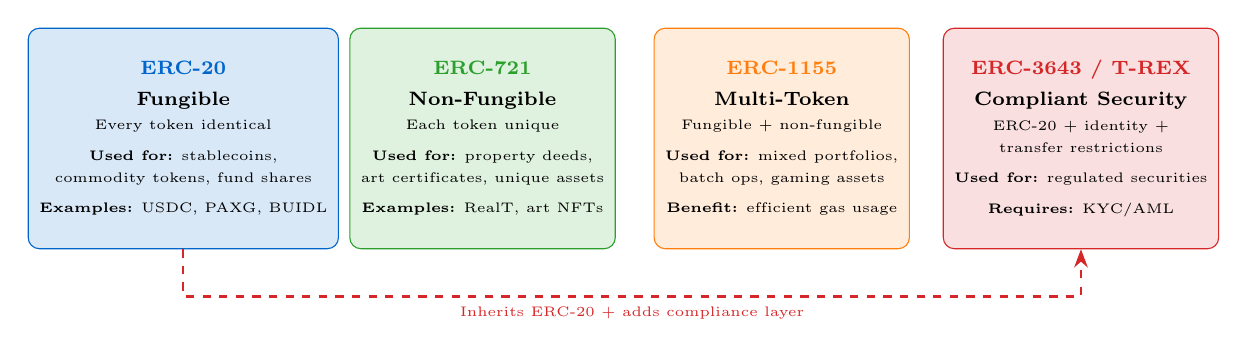
\begin{tikzpicture}[
  rwacard/.style={draw,rounded corners=4pt,minimum width=3.2cm,minimum height=2.8cm,
    align=center,font=\scriptsize,inner sep=4pt},
  rwainherit/.style={-{Stealth},thick,dashed,mlred}
]
  % ERC-20
  \node[rwacard,fill=mlblue!15,draw=mlblue,text=black] (e20) at (0,0) {
    {\color{mlblue}\textbf{ERC-20}}\\[3pt]
    \textbf{Fungible}\\[1pt]
    \tiny Every token identical\\[3pt]
    \tiny \textbf{Used for:} stablecoins,\\
    \tiny commodity tokens, fund shares\\[3pt]
    \tiny \textbf{Examples:} USDC, PAXG, BUIDL};
  % ERC-721
  \node[rwacard,fill=mlgreen!15,draw=mlgreen,text=black] (e721) at (3.8,0) {
    {\color{mlgreen}\textbf{ERC-721}}\\[3pt]
    \textbf{Non-Fungible}\\[1pt]
    \tiny Each token unique\\[3pt]
    \tiny \textbf{Used for:} property deeds,\\
    \tiny art certificates, unique assets\\[3pt]
    \tiny \textbf{Examples:} RealT, art NFTs};
  % ERC-1155
  \node[rwacard,fill=mlorange!15,draw=mlorange,text=black] (e1155) at (7.6,0) {
    {\color{mlorange}\textbf{ERC-1155}}\\[3pt]
    \textbf{Multi-Token}\\[1pt]
    \tiny Fungible + non-fungible\\[3pt]
    \tiny \textbf{Used for:} mixed portfolios,\\
    \tiny batch ops, gaming assets\\[3pt]
    \tiny \textbf{Benefit:} efficient gas usage};
  % ERC-3643
  \node[rwacard,fill=mlred!15,draw=mlred,text=black] (e3643) at (11.4,0) {
    {\color{mlred}\textbf{ERC-3643 / T-REX}}\\[3pt]
    \textbf{Compliant Security}\\[1pt]
    \tiny ERC-20 + identity +\\
    \tiny transfer restrictions\\[3pt]
    \tiny \textbf{Used for:} regulated securities\\[3pt]
    \tiny \textbf{Requires:} KYC/AML};
  % Inheritance arrow from ERC-20 to ERC-3643
  \draw[rwainherit] (e20.south) -- ++(0,-0.6) -| node[pos=0.25,below,font=\tiny\color{mlred}]
    {Inherits ERC-20 + adds compliance layer} (e3643.south);
\end{tikzpicture}
\bottomnote{ERC-3643 is the standard adopted by most security token platforms -- it adds identity verification and transfer restrictions to ERC-20}
\end{frame}

% Frame 8: ERC-20 Asset Token Contract
\begin{frame}[fragile]{ERC-20 Asset Token Contract}
\begin{columns}[T]
\column{0.48\textwidth}
\begin{lstlisting}
// Tokenized Real Estate Fund
contract RealEstateFund {
    string public name =
        "NYC Property Fund";
    string public symbol = "NYCPF";
    uint8 public decimals = 18;
    uint256 public totalSupply;

    mapping(address => uint256)
        public balanceOf;

    address public manager;
    uint256 public navPerToken;

    constructor(uint256 supply) {
        manager = msg.sender;
        totalSupply = supply;
        balanceOf[msg.sender] = supply;
    }

    function updateNAV(
        uint256 newNAV
    ) external {
        require(msg.sender == manager);
        navPerToken = newNAV;
        emit NAVUpdated(newNAV);
    }
}
\end{lstlisting}

\column{0.48\textwidth}
\vspace{2mm}
\begin{block}{How This Works}
\footnotesize
\begin{itemize}
  \item \textbf{Token = Fund Share}: Each token represents a fractional ownership share in the NYC Property Fund
  \item \textbf{NAV Updates}: Fund manager calls \texttt{updateNAV()} to reflect current property valuation
  \item \textbf{balanceOf}: Tracks each investor's fractional ownership on-chain
  \item \textbf{Transfer}: Standard ERC-20 transfer enables secondary market trading 24/7
  \item \textbf{Dividends}: Rental income distributed via a separate distribution function (not shown)
\end{itemize}
\end{block}
\vspace{2mm}
\begin{block}{Key Design Patterns}
\footnotesize
\begin{itemize}
  \item Manager role for privileged operations
  \item On-chain state reflects off-chain asset value
  \item Transparent, auditable ownership ledger
\end{itemize}
\end{block}
\end{columns}
\bottomnote{This simplified contract shows the core pattern: tokens represent ownership shares, manager updates NAV, holders can transfer freely}
\end{frame}

% Frame 9: Fractionalization Mechanics
\begin{frame}{Fractionalization Mechanics}
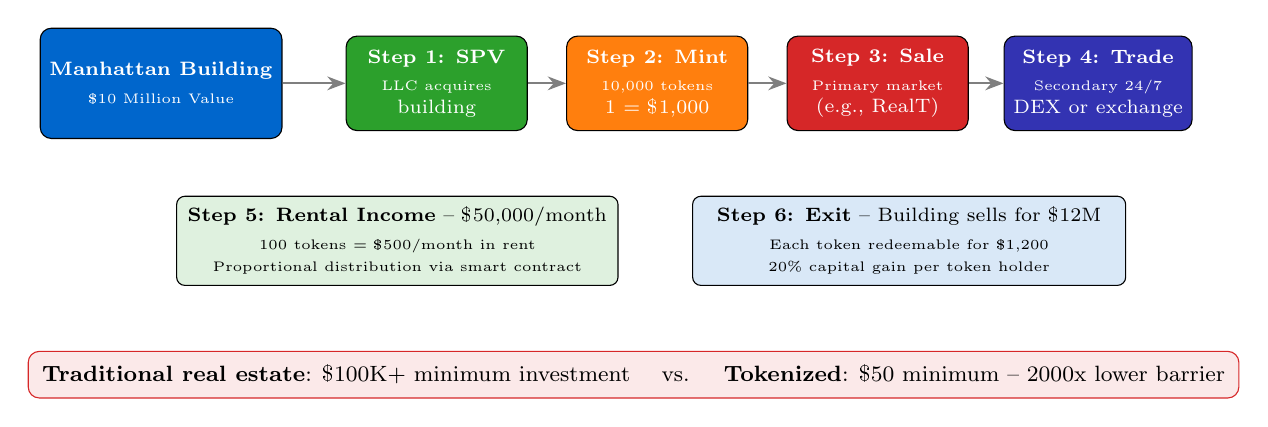
\begin{tikzpicture}[
  rwanode/.style={draw,rounded corners=4pt,minimum width=2.3cm,minimum height=1.2cm,
    align=center,font=\scriptsize,text=white},
  rwaarrow/.style={-{Stealth},thick,mlgray}
]
  % Asset
  \node[rwanode,fill=mlblue,minimum width=3.0cm,minimum height=1.4cm] (asset) at (0,0.5) {
    \textbf{Manhattan Building}\\[2pt]\tiny \$10 Million Value};
  % Steps
  \node[rwanode,fill=mlgreen] (s1) at (3.5,0.5) {\textbf{Step 1: SPV}\\[2pt]\tiny LLC acquires\\building};
  \node[rwanode,fill=mlorange] (s2) at (6.3,0.5) {\textbf{Step 2: Mint}\\[2pt]\tiny 10,000 tokens\\1 = \$1,000};
  \node[rwanode,fill=mlred] (s3) at (9.1,0.5) {\textbf{Step 3: Sale}\\[2pt]\tiny Primary market\\(e.g., RealT)};
  \node[rwanode,fill=mlpurple] (s4) at (11.9,0.5) {\textbf{Step 4: Trade}\\[2pt]\tiny Secondary 24/7\\DEX or exchange};
  % Arrows
  \draw[rwaarrow] (asset.east) -- (s1.west);
  \draw[rwaarrow] (s1.east) -- (s2.west);
  \draw[rwaarrow] (s2.east) -- (s3.west);
  \draw[rwaarrow] (s3.east) -- (s4.west);
  % Income and exit boxes
  \node[draw,fill=mlgreen!15,rounded corners=3pt,minimum width=5.5cm,align=center,font=\scriptsize,inner sep=4pt]
    (income) at (3.0,-1.5) {\textbf{Step 5: Rental Income} -- \$50,000/month\\[2pt]
    \tiny 100 tokens = \$500/month in rent\\
    \tiny Proportional distribution via smart contract};
  \node[draw,fill=mlblue!15,rounded corners=3pt,minimum width=5.5cm,align=center,font=\scriptsize,inner sep=4pt]
    (exit) at (9.5,-1.5) {\textbf{Step 6: Exit} -- Building sells for \$12M\\[2pt]
    \tiny Each token redeemable for \$1,200\\
    \tiny 20\% capital gain per token holder};
  % Comparison callout
  \node[draw=mlred,fill=mlred!10,rounded corners=4pt,minimum width=12.0cm,align=center,font=\footnotesize,inner sep=5pt]
    at (6.0,-3.2) {\textbf{Traditional real estate}: \$100K+ minimum investment \quad vs. \quad
    \textbf{Tokenized}: \$50 minimum -- 2000x lower barrier};
\end{tikzpicture}
\bottomnote{Fractionalization is the most transformative aspect of tokenization -- it turns illiquid assets into liquid, accessible investments}
\end{frame}

% Frame 10: Benefits of Tokenization
\begin{frame}{Benefits of Tokenization}
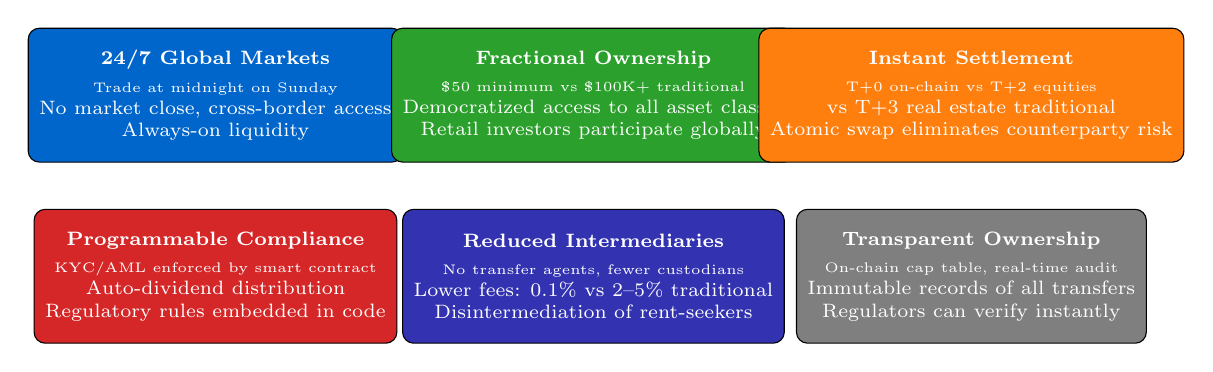
\begin{tikzpicture}[
  rwabenefit/.style={draw,rounded corners=4pt,minimum width=4.3cm,minimum height=1.7cm,
    align=center,font=\scriptsize,text=white,inner sep=4pt}
]
  % Row 1
  \node[rwabenefit,fill=mlblue] at (0,0) {\textbf{24/7 Global Markets}\\[2pt]
    \tiny Trade at midnight on Sunday\\No market close, cross-border access\\Always-on liquidity};
  \node[rwabenefit,fill=mlgreen] at (4.8,0) {\textbf{Fractional Ownership}\\[2pt]
    \tiny \$50 minimum vs \$100K+ traditional\\Democratized access to all asset classes\\Retail investors participate globally};
  \node[rwabenefit,fill=mlorange] at (9.6,0) {\textbf{Instant Settlement}\\[2pt]
    \tiny T+0 on-chain vs T+2 equities\\vs T+3 real estate traditional\\Atomic swap eliminates counterparty risk};
  % Row 2
  \node[rwabenefit,fill=mlred] at (0,-2.3) {\textbf{Programmable Compliance}\\[2pt]
    \tiny KYC/AML enforced by smart contract\\Auto-dividend distribution\\Regulatory rules embedded in code};
  \node[rwabenefit,fill=mlpurple] at (4.8,-2.3) {\textbf{Reduced Intermediaries}\\[2pt]
    \tiny No transfer agents, fewer custodians\\Lower fees: 0.1\% vs 2--5\% traditional\\Disintermediation of rent-seekers};
  \node[rwabenefit,fill=mlgray] at (9.6,-2.3) {\textbf{Transparent Ownership}\\[2pt]
    \tiny On-chain cap table, real-time audit\\Immutable records of all transfers\\Regulators can verify instantly};
\end{tikzpicture}
\bottomnote{McKinsey estimates tokenization could save financial institutions \$100--200B annually in back-office costs alone}
\end{frame}

% Frame 11: Challenges of Tokenization
\begin{frame}{Challenges of Tokenization}
\begin{columns}[T]
\column{0.48\textwidth}
\begin{block}{Technical Challenges}
\footnotesize
\begin{itemize}
  \item \textbf{Oracle Problem}: How does the blockchain know the building's condition, occupancy, or sale price?
  \item \textbf{Smart Contract Risk}: Bugs can lock or drain tokenized assets worth millions
  \item \textbf{Scalability}: High-value assets need robust, battle-tested chains
  \item \textbf{Interoperability}: Tokenized assets on different chains cannot easily interact
\end{itemize}
\end{block}

\column{0.48\textwidth}
\begin{block}{Legal \& Regulatory Challenges}
\footnotesize
\begin{itemize}
  \item \textbf{Legal Recognition}: Does a token convey legal ownership? Varies by jurisdiction
  \item \textbf{Cross-Border Complexity}: US-tokenized building sold to Japanese investor -- which laws apply?
  \item \textbf{Bankruptcy}: If the SPV or platform fails, what happens to token holders?
  \item \textbf{Tax Reporting}: Capital gains, rental income, cross-border withholding
\end{itemize}
\end{block}
\end{columns}
\vspace{3mm}
\centering
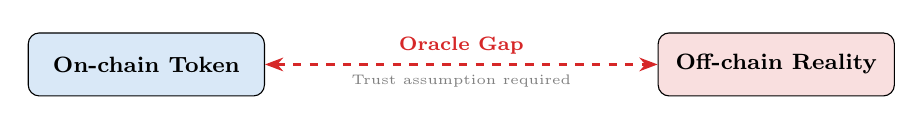
\begin{tikzpicture}
  \node[draw,fill=mlblue!15,rounded corners=4pt,minimum width=3.0cm,minimum height=0.8cm,
    align=center,font=\footnotesize\bfseries] (onchain) at (0,0) {On-chain Token};
  \node[draw,fill=mlred!15,rounded corners=4pt,minimum width=3.0cm,minimum height=0.8cm,
    align=center,font=\footnotesize\bfseries] (offchain) at (8,0) {Off-chain Reality};
  \draw[{Stealth}-{Stealth},thick,dashed,mlred] (onchain.east) -- node[above,font=\scriptsize\bfseries,mlred]
    {Oracle Gap} node[below,font=\tiny,mlgray] {Trust assumption required} (offchain.west);
\end{tikzpicture}
\bottomnote{The oracle problem is fundamental: a blockchain can verify on-chain state perfectly, but cannot independently verify off-chain reality}
\end{frame}

% Frame 12: The Oracle Problem for RWA
\begin{frame}{The Oracle Problem for RWA}
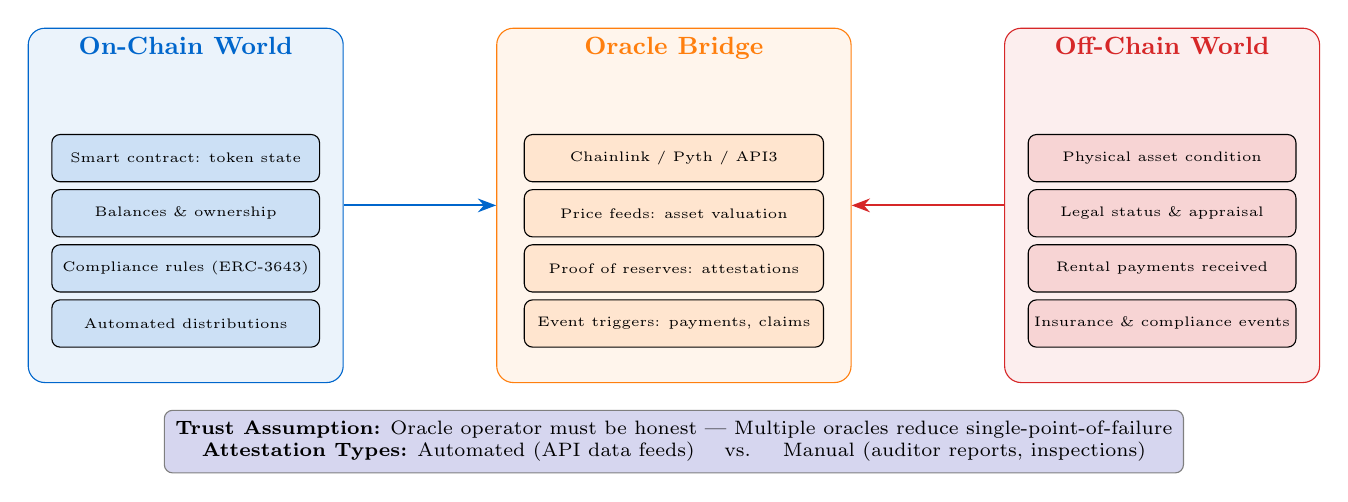
\begin{tikzpicture}[
  rwazone/.style={draw,rounded corners=6pt,minimum width=4.0cm,minimum height=4.5cm,
    align=center,inner sep=6pt},
  rwaitem/.style={draw,rounded corners=3pt,minimum width=3.4cm,minimum height=0.6cm,
    align=center,font=\tiny,inner sep=2pt}
]
  % On-chain zone
  \node[rwazone,fill=mlblue!8,draw=mlblue] (onzone) at (0,0) {};
  \node[font=\small\bfseries,mlblue,anchor=north] at (onzone.north) {On-Chain World};
  \node[rwaitem,fill=mlblue!20] (oc1) at (0,0.6) {Smart contract: token state};
  \node[rwaitem,fill=mlblue!20] (oc2) at (0,-0.1) {Balances \& ownership};
  \node[rwaitem,fill=mlblue!20] (oc3) at (0,-0.8) {Compliance rules (ERC-3643)};
  \node[rwaitem,fill=mlblue!20] (oc4) at (0,-1.5) {Automated distributions};

  % Oracle bridge (center)
  \node[rwazone,fill=mlorange!8,draw=mlorange,minimum width=4.5cm] (bridge) at (6.2,0) {};
  \node[font=\small\bfseries,mlorange,anchor=north] at (bridge.north) {Oracle Bridge};
  \node[rwaitem,fill=mlorange!20,minimum width=3.8cm] (br1) at (6.2,0.6) {Chainlink / Pyth / API3};
  \node[rwaitem,fill=mlorange!20,minimum width=3.8cm] (br2) at (6.2,-0.1) {Price feeds: asset valuation};
  \node[rwaitem,fill=mlorange!20,minimum width=3.8cm] (br3) at (6.2,-0.8) {Proof of reserves: attestations};
  \node[rwaitem,fill=mlorange!20,minimum width=3.8cm] (br4) at (6.2,-1.5) {Event triggers: payments, claims};

  % Off-chain zone
  \node[rwazone,fill=mlred!8,draw=mlred] (offzone) at (12.4,0) {};
  \node[font=\small\bfseries,mlred,anchor=north] at (offzone.north) {Off-Chain World};
  \node[rwaitem,fill=mlred!20] (of1) at (12.4,0.6) {Physical asset condition};
  \node[rwaitem,fill=mlred!20] (of2) at (12.4,-0.1) {Legal status \& appraisal};
  \node[rwaitem,fill=mlred!20] (of3) at (12.4,-0.8) {Rental payments received};
  \node[rwaitem,fill=mlred!20] (of4) at (12.4,-1.5) {Insurance \& compliance events};

  % Arrows between zones
  \draw[-{Stealth},thick,mlblue] (onzone.east) -- (bridge.west);
  \draw[-{Stealth},thick,mlred] (offzone.west) -- (bridge.east);

  % Trust assumption
  \node[draw=mlgray,fill=mllavender4,rounded corners=3pt,minimum width=12.0cm,align=center,
    font=\scriptsize,inner sep=4pt] at (6.2,-3.0) {
    \textbf{Trust Assumption:} Oracle operator must be honest | Multiple oracles reduce single-point-of-failure\\
    \textbf{Attestation Types:} Automated (API data feeds) \quad vs. \quad Manual (auditor reports, inspections)};
\end{tikzpicture}
\bottomnote{Unlike DeFi protocols that use on-chain price feeds, RWA oracles often require human attestation -- introducing trust assumptions}
\end{frame}

% Frame 13: Tokenization Market Map
\begin{frame}{Tokenization Market Map}
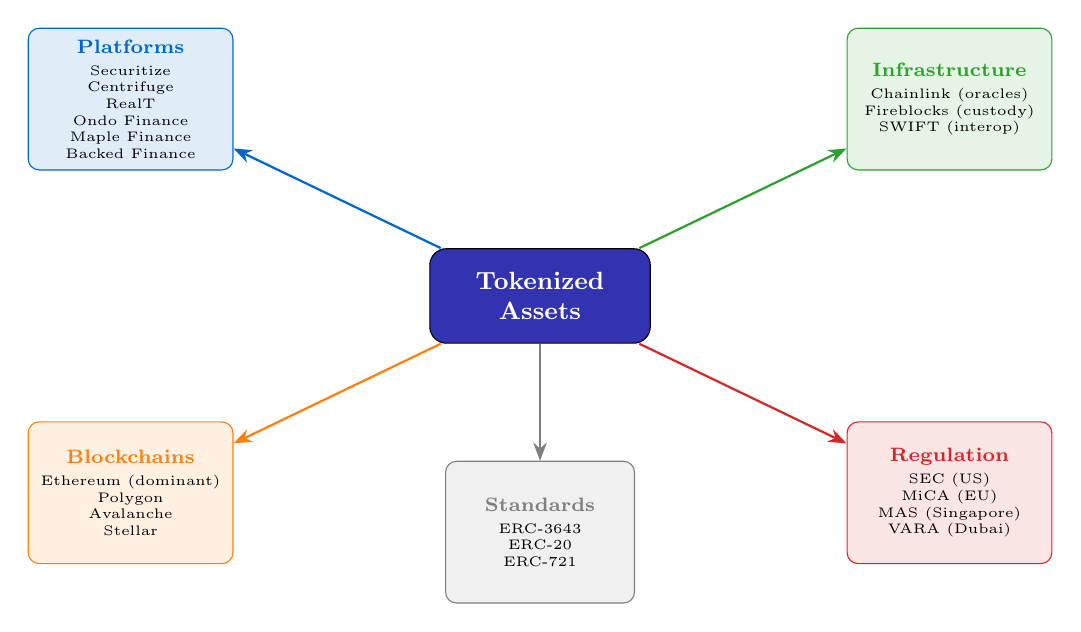
\begin{tikzpicture}[
  rwahub/.style={draw,fill=mlpurple,text=white,rounded corners=6pt,
    minimum width=2.8cm,minimum height=1.2cm,align=center,font=\small\bfseries},
  rwaspoke/.style={draw,rounded corners=4pt,minimum width=2.6cm,minimum height=1.8cm,
    align=center,font=\tiny,inner sep=3pt}
]
  % Center hub
  \node[rwahub] (hub) at (6.2,0) {Tokenized\\Assets};

  % Platforms (top-left)
  \node[rwaspoke,fill=mlblue!12,draw=mlblue] (plat) at (1.0,2.5) {
    {\scriptsize\bfseries\color{mlblue}Platforms}\\[2pt]
    Securitize\\Centrifuge\\RealT\\Ondo Finance\\Maple Finance\\Backed Finance};

  % Infrastructure (top-right)
  \node[rwaspoke,fill=mlgreen!12,draw=mlgreen] (infra) at (11.4,2.5) {
    {\scriptsize\bfseries\color{mlgreen}Infrastructure}\\[2pt]
    Chainlink (oracles)\\Fireblocks (custody)\\SWIFT (interop)};

  % Blockchains (bottom-left)
  \node[rwaspoke,fill=mlorange!12,draw=mlorange] (chains) at (1.0,-2.5) {
    {\scriptsize\bfseries\color{mlorange}Blockchains}\\[2pt]
    Ethereum (dominant)\\Polygon\\Avalanche\\Stellar};

  % Regulation (bottom-right)
  \node[rwaspoke,fill=mlred!12,draw=mlred] (reg) at (11.4,-2.5) {
    {\scriptsize\bfseries\color{mlred}Regulation}\\[2pt]
    SEC (US)\\MiCA (EU)\\MAS (Singapore)\\VARA (Dubai)};

  % Standards (bottom-center)
  \node[rwaspoke,fill=mlgray!12,draw=mlgray,minimum width=2.4cm] (std) at (6.2,-3.0) {
    {\scriptsize\bfseries\color{mlgray}Standards}\\[2pt]
    ERC-3643\\ERC-20\\ERC-721};

  % Arrows from hub to spokes
  \draw[-{Stealth},thick,mlblue] (hub) -- (plat);
  \draw[-{Stealth},thick,mlgreen] (hub) -- (infra);
  \draw[-{Stealth},thick,mlorange] (hub) -- (chains);
  \draw[-{Stealth},thick,mlred] (hub) -- (reg);
  \draw[-{Stealth},thick,mlgray] (hub) -- (std);
\end{tikzpicture}
\bottomnote{Ethereum dominates RWA tokenization with 60\%+ market share -- security, liquidity, and institutional trust drive this concentration}
\end{frame}

% Frame 14: Section 1 Summary
\begin{frame}{Section 1 Summary: Tokenization Fundamentals}
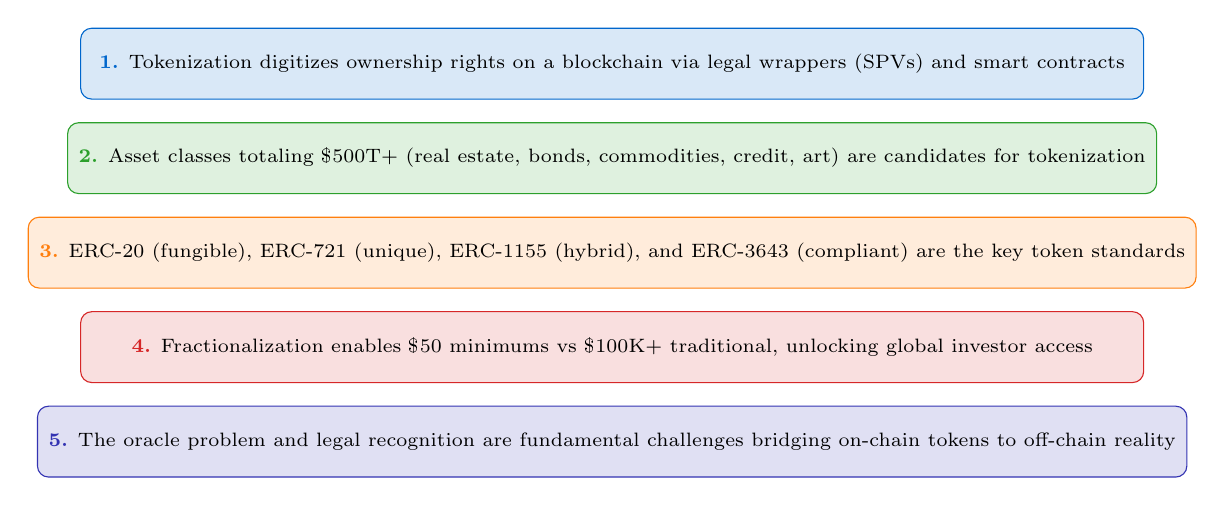
\begin{tikzpicture}[
  rwasummary/.style={draw,rounded corners=4pt,minimum width=13.5cm,minimum height=0.9cm,
    align=center,font=\scriptsize,inner sep=4pt}
]
  \node[rwasummary,fill=mlblue!15,draw=mlblue] at (6.5,2.0) {
    {\color{mlblue}\textbf{1.}} Tokenization digitizes ownership rights on a blockchain via legal wrappers (SPVs) and smart contracts};
  \node[rwasummary,fill=mlgreen!15,draw=mlgreen] at (6.5,0.8) {
    {\color{mlgreen}\textbf{2.}} Asset classes totaling \$500T+ (real estate, bonds, commodities, credit, art) are candidates for tokenization};
  \node[rwasummary,fill=mlorange!15,draw=mlorange] at (6.5,-0.4) {
    {\color{mlorange}\textbf{3.}} ERC-20 (fungible), ERC-721 (unique), ERC-1155 (hybrid), and ERC-3643 (compliant) are the key token standards};
  \node[rwasummary,fill=mlred!15,draw=mlred] at (6.5,-1.6) {
    {\color{mlred}\textbf{4.}} Fractionalization enables \$50 minimums vs \$100K+ traditional, unlocking global investor access};
  \node[rwasummary,fill=mlpurple!15,draw=mlpurple] at (6.5,-2.8) {
    {\color{mlpurple}\textbf{5.}} The oracle problem and legal recognition are fundamental challenges bridging on-chain tokens to off-chain reality};
\end{tikzpicture}
\bottomnote{Section 1 complete | Next: Section 2 -- Stablecoins Deep Dive}
\end{frame}

%% ============================================================
%% SECTION 2: STABLECOINS DEEP DIVE
%% ============================================================
\section{Stablecoins Deep Dive}

% Frame 15: Section 2 Divider
\begin{frame}{}
\begin{beamercolorbox}[sep=12pt,center,rounded=true,shadow=true]{palette quaternary}
  {\Large\bfseries Section 2: Stablecoins Deep Dive}\\[6pt]
  {\normalsize Taxonomy, mechanics, reserves, risks, and the regulatory frontier}
\end{beamercolorbox}
\vspace{4mm}
\begin{columns}[T]
\column{0.5\textwidth}
\begin{block}{What You Will Learn}
\footnotesize
\begin{itemize}
  \item Stablecoin taxonomy: fiat-backed, crypto-backed, algorithmic, commodity-backed
  \item USDT, USDC, and DAI mechanics in depth
  \item Reserve attestation models and depeg risks
  \item The Terra/Luna collapse and regulatory response
\end{itemize}
\end{block}
\column{0.5\textwidth}
\begin{block}{Frames in This Section}
\footnotesize
\begin{itemize}
  \item Frame 16: Stablecoin Taxonomy
  \item Frame 17: USDT (Tether) Mechanics
  \item Frame 18: USDC \& Reserve Transparency
  \item Frame 19: DAI \& Crypto-Backed Mechanics
  \item Frame 20: Collateralized Vault Contract (Code)
  \item Frame 21: The Terra/Luna Collapse
  \item Frame 22: Stablecoin Reserve Models Compared
  \item Frame 23: Stablecoin Market Dominance
  \item Frame 24: Stablecoin Regulation
  \item Frame 25: Section 2 Summary
\end{itemize}
\end{block}
\end{columns}
\bottomnote{Section 2 of 5 | Frames 15--25}
\end{frame}

% Frame 16: Stablecoin Taxonomy
\begin{frame}{Stablecoin Taxonomy}
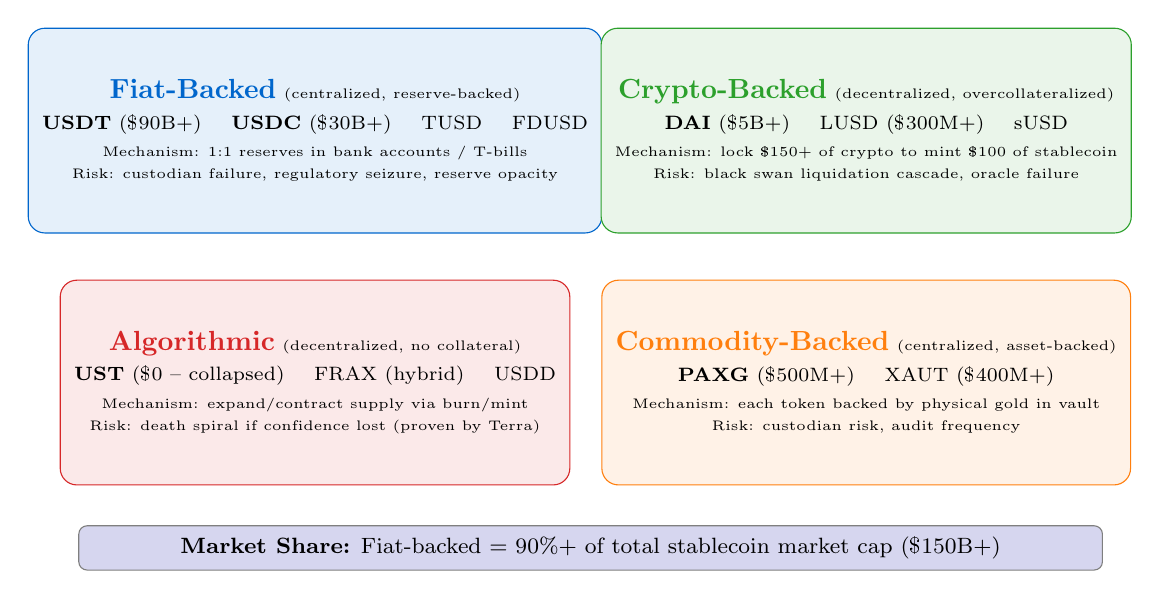
\begin{tikzpicture}[
  rwaquad/.style={draw,rounded corners=6pt,minimum width=6.4cm,minimum height=2.6cm,
    align=center,font=\scriptsize,inner sep=5pt},
  rwatag/.style={font=\tiny,align=center}
]
  % Quadrant 1: Fiat-Backed (top-left)
  \node[rwaquad,fill=mlblue!10,draw=mlblue] (q1) at (0,1.5) {
    {\normalsize\bfseries\color{mlblue}Fiat-Backed} {\tiny (centralized, reserve-backed)}\\[3pt]
    \textbf{USDT} (\$90B+) \quad \textbf{USDC} (\$30B+) \quad TUSD \quad FDUSD\\[2pt]
    \tiny Mechanism: 1:1 reserves in bank accounts / T-bills\\
    \tiny Risk: custodian failure, regulatory seizure, reserve opacity};
  % Quadrant 2: Crypto-Backed (top-right)
  \node[rwaquad,fill=mlgreen!10,draw=mlgreen] (q2) at (7.0,1.5) {
    {\normalsize\bfseries\color{mlgreen}Crypto-Backed} {\tiny (decentralized, overcollateralized)}\\[3pt]
    \textbf{DAI} (\$5B+) \quad LUSD (\$300M+) \quad sUSD\\[2pt]
    \tiny Mechanism: lock \$150+ of crypto to mint \$100 of stablecoin\\
    \tiny Risk: black swan liquidation cascade, oracle failure};
  % Quadrant 3: Algorithmic (bottom-left)
  \node[rwaquad,fill=mlred!10,draw=mlred] (q3) at (0,-1.7) {
    {\normalsize\bfseries\color{mlred}Algorithmic} {\tiny (decentralized, no collateral)}\\[3pt]
    \textbf{UST} (\$0 -- collapsed) \quad FRAX (hybrid) \quad USDD\\[2pt]
    \tiny Mechanism: expand/contract supply via burn/mint\\
    \tiny Risk: death spiral if confidence lost (proven by Terra)};
  % Quadrant 4: Commodity-Backed (bottom-right)
  \node[rwaquad,fill=mlorange!10,draw=mlorange] (q4) at (7.0,-1.7) {
    {\normalsize\bfseries\color{mlorange}Commodity-Backed} {\tiny (centralized, asset-backed)}\\[3pt]
    \textbf{PAXG} (\$500M+) \quad XAUT (\$400M+)\\[2pt]
    \tiny Mechanism: each token backed by physical gold in vault\\
    \tiny Risk: custodian risk, audit frequency};
  % Market share annotation
  \node[draw=mlgray,fill=mllavender4,rounded corners=3pt,minimum width=13.0cm,align=center,
    font=\footnotesize,inner sep=4pt] at (3.5,-3.8) {
    \textbf{Market Share:} Fiat-backed = 90\%+ of total stablecoin market cap (\$150B+)};
\end{tikzpicture}
\bottomnote{Stablecoins are the largest crypto use case by settlement volume -- fiat-backed stablecoins dominate with over 90\% market share}
\end{frame}

% Frame 17: USDT (Tether) Mechanics
\begin{frame}{USDT (Tether) Mechanics}
\begin{columns}[T]
\column{0.46\textwidth}
\begin{block}{How Tether Works}
\footnotesize
\begin{itemize}
  \item \textbf{Market cap:} \$90B+ (largest stablecoin)
  \item \textbf{Issuer:} Tether Limited (BVI)
  \item \textbf{Peg:} Authorized participants deposit USD, receive USDT; redeem USDT for USD
  \item \textbf{Reserve composition} (latest attestation):
    \begin{itemize}\scriptsize
      \item $\sim$85\% US Treasury bills
      \item $\sim$10\% secured loans
      \item $\sim$5\% other (BTC, precious metals)
    \end{itemize}
  \item \textbf{Controversy:} 2019 NYAG investigation, undisclosed \$850M Bitfinex loan
  \item \textbf{No full audit} -- quarterly attestation by BDO Italia
\end{itemize}
\end{block}

\column{0.50\textwidth}
\vspace{1mm}
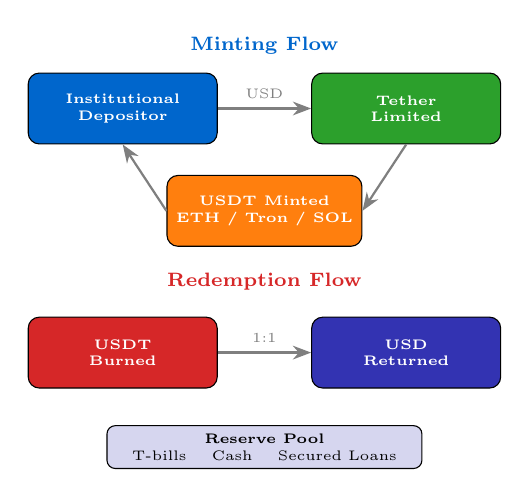
\begin{tikzpicture}[
  rwaflow/.style={draw,rounded corners=4pt,minimum width=2.4cm,minimum height=0.9cm,
    align=center,font=\tiny\bfseries,text=white},
  rwaflowarr/.style={-{Stealth},thick,mlgray}
]
  % Mint flow
  \node[font=\scriptsize\bfseries,mlblue] at (1.8,3.0) {Minting Flow};
  \node[rwaflow,fill=mlblue] (dep) at (0,2.2) {Institutional\\Depositor};
  \node[rwaflow,fill=mlgreen] (tether) at (3.6,2.2) {Tether\\Limited};
  \node[rwaflow,fill=mlorange] (mint) at (1.8,0.9) {USDT Minted\\ETH / Tron / SOL};
  \draw[rwaflowarr] (dep.east) -- node[above,font=\tiny] {USD} (tether.west);
  \draw[rwaflowarr] (tether.south) -- (mint.east);
  \draw[rwaflowarr] (mint.west) -- (dep.south);
  % Redemption flow
  \node[font=\scriptsize\bfseries,mlred] at (1.8,0.0) {Redemption Flow};
  \node[rwaflow,fill=mlred] (burn) at (0,-0.9) {USDT\\Burned};
  \node[rwaflow,fill=mlpurple] (usdret) at (3.6,-0.9) {USD\\Returned};
  \draw[rwaflowarr] (burn.east) -- node[above,font=\tiny] {1:1} (usdret.west);
  % Reserve pool
  \node[draw,fill=mllavender4,rounded corners=3pt,minimum width=4.0cm,align=center,
    font=\tiny,inner sep=3pt] at (1.8,-2.1) {
    \textbf{Reserve Pool}\\T-bills \quad Cash \quad Secured Loans};
\end{tikzpicture}
\end{columns}
\bottomnote{Tether is the most systemically important stablecoin but also the most controversial -- \$90B+ in circulation, never fully audited}
\end{frame}

% Frame 18: USDC & Reserve Transparency
\begin{frame}{USDC \& Reserve Transparency}
\begin{columns}[T]
\column{0.46\textwidth}
\begin{block}{How Circle/USDC Works}
\footnotesize
\begin{itemize}
  \item \textbf{Market cap:} \$30B+ (second largest)
  \item \textbf{Issuer:} Circle (US-regulated money transmitter)
  \item \textbf{Reserves:} $\sim$80\% short-term US Treasuries, $\sim$20\% cash at regulated banks
  \item \textbf{Monthly attestation} by Deloitte (Big 4 auditor)
  \item \textbf{Regulated} in US, EU (MiCA compliant), Singapore
  \item \textbf{March 2023 depeg:} SVB held \$3.3B of reserves -- depeg to \$0.87 during collapse, recovered in 48h when Fed backstopped deposits
\end{itemize}
\end{block}

\column{0.50\textwidth}
\vspace{1mm}
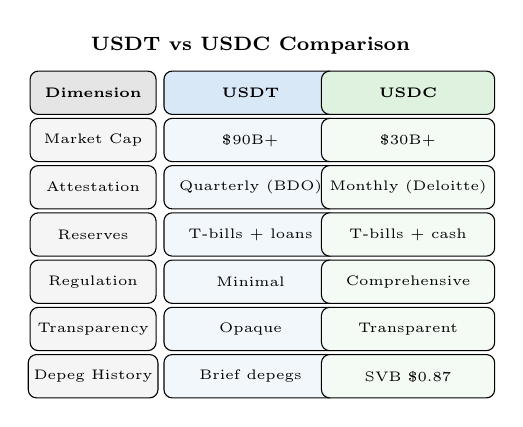
\begin{tikzpicture}[
  rwacomp/.style={draw,rounded corners=3pt,minimum width=2.2cm,minimum height=0.55cm,
    align=center,font=\tiny,inner sep=2pt}
]
  \node[font=\scriptsize\bfseries] at (2.0,3.2) {USDT vs USDC Comparison};
  % Headers
  \node[rwacomp,fill=mlgray!20,minimum width=1.6cm] at (0,2.6) {\textbf{Dimension}};
  \node[rwacomp,fill=mlblue!15] at (2.0,2.6) {\textbf{USDT}};
  \node[rwacomp,fill=mlgreen!15] at (4.0,2.6) {\textbf{USDC}};
  % Rows
  \node[rwacomp,fill=mlgray!8,minimum width=1.6cm] at (0,2.0) {Market Cap};
  \node[rwacomp,fill=mlblue!5] at (2.0,2.0) {\$90B+};
  \node[rwacomp,fill=mlgreen!5] at (4.0,2.0) {\$30B+};

  \node[rwacomp,fill=mlgray!8,minimum width=1.6cm] at (0,1.4) {Attestation};
  \node[rwacomp,fill=mlblue!5] at (2.0,1.4) {Quarterly (BDO)};
  \node[rwacomp,fill=mlgreen!5] at (4.0,1.4) {Monthly (Deloitte)};

  \node[rwacomp,fill=mlgray!8,minimum width=1.6cm] at (0,0.8) {Reserves};
  \node[rwacomp,fill=mlblue!5] at (2.0,0.8) {T-bills + loans};
  \node[rwacomp,fill=mlgreen!5] at (4.0,0.8) {T-bills + cash};

  \node[rwacomp,fill=mlgray!8,minimum width=1.6cm] at (0,0.2) {Regulation};
  \node[rwacomp,fill=mlblue!5] at (2.0,0.2) {Minimal};
  \node[rwacomp,fill=mlgreen!5] at (4.0,0.2) {Comprehensive};

  \node[rwacomp,fill=mlgray!8,minimum width=1.6cm] at (0,-0.4) {Transparency};
  \node[rwacomp,fill=mlblue!5] at (2.0,-0.4) {Opaque};
  \node[rwacomp,fill=mlgreen!5] at (4.0,-0.4) {Transparent};

  \node[rwacomp,fill=mlgray!8,minimum width=1.6cm] at (0,-1.0) {Depeg History};
  \node[rwacomp,fill=mlblue!5] at (2.0,-1.0) {Brief depegs};
  \node[rwacomp,fill=mlgreen!5] at (4.0,-1.0) {SVB \$0.87};
\end{tikzpicture}
\end{columns}
\bottomnote{The SVB depeg showed that even well-reserved stablecoins face risk from banking system failures -- diversification of reserves matters}
\end{frame}

% Frame 19: DAI & Crypto-Backed Mechanics
\begin{frame}{DAI \& Crypto-Backed Mechanics}
\begin{columns}[T]
\column{0.46\textwidth}
\begin{block}{MakerDAO/DAI Architecture}
\footnotesize
\begin{itemize}
  \item \textbf{Decentralized stablecoin:} no single issuer
  \item \textbf{Vault (CDP) mechanism:}
    \begin{itemize}\scriptsize
      \item Deposit ETH (or WBTC, stETH) as collateral
      \item Mint DAI up to collateralization ratio (e.g., 150\% for ETH)
      \item Pay stability fee (interest) on outstanding DAI
      \item If collateral ratio drops below threshold, liquidation auction
    \end{itemize}
  \item \textbf{Governance:} MKR token holders set parameters (rates, ratios, collateral types)
  \item \textbf{PSM:} Peg Stability Module allows 1:1 swap with USDC
  \item \textbf{RWA vaults:} \$2B+ in real-world assets (US Treasuries, commercial loans)
\end{itemize}
\end{block}

\column{0.50\textwidth}
\vspace{1mm}
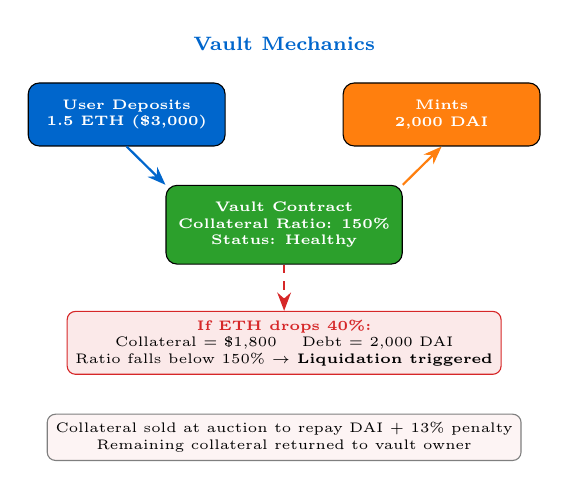
\begin{tikzpicture}[
  rwavault/.style={draw,rounded corners=4pt,minimum width=2.5cm,minimum height=0.8cm,
    align=center,font=\tiny\bfseries,text=white},
  rwavaultarr/.style={-{Stealth},thick}
]
  \node[font=\scriptsize\bfseries,mlblue] at (2.0,3.2) {Vault Mechanics};
  % User deposits
  \node[rwavault,fill=mlblue] (user) at (0,2.3) {User Deposits\\1.5 ETH (\$3,000)};
  \node[rwavault,fill=mlgreen,minimum width=3.0cm,minimum height=1.0cm] (vault) at (2.0,0.9) {Vault Contract\\{\tiny Collateral Ratio: 150\%}\\{\tiny Status: Healthy}};
  \node[rwavault,fill=mlorange] (dai) at (4.0,2.3) {Mints\\2,000 DAI};
  % Arrows
  \draw[rwavaultarr,mlblue] (user.south) -- (vault.north west);
  \draw[rwavaultarr,mlorange] (vault.north east) -- (dai.south);
  % Liquidation scenario
  \node[draw,fill=mlred!10,draw=mlred,rounded corners=3pt,minimum width=4.5cm,align=center,
    font=\tiny,inner sep=3pt] (liq) at (2.0,-0.6) {
    \textbf{\color{mlred}If ETH drops 40\%:}\\
    Collateral = \$1,800 \quad Debt = 2,000 DAI\\
    Ratio falls below 150\% $\rightarrow$ \textbf{Liquidation triggered}};
  \draw[rwavaultarr,mlred,dashed] (vault.south) -- (liq.north);
  % Liquidation result
  \node[draw,fill=mlred!5,draw=mlgray,rounded corners=3pt,minimum width=4.5cm,align=center,
    font=\tiny,inner sep=3pt] at (2.0,-1.8) {
    Collateral sold at auction to repay DAI + 13\% penalty\\
    Remaining collateral returned to vault owner};
\end{tikzpicture}
\end{columns}
\bottomnote{MakerDAO's pivot to RWA collateral is historic: DAI is now backed 40\%+ by real-world assets, blurring the line between DeFi and TradFi}
\end{frame}

% Frame 20: Collateralized Vault Contract [CODE FRAME 2]
\begin{frame}[fragile]{Collateralized Vault Contract}
\begin{columns}[T]
\column{0.48\textwidth}
\begin{lstlisting}
// Simplified Collateral Vault
contract StablecoinVault {
    uint256 public constant
        MIN_RATIO = 150; // 150%
    mapping(address => uint256)
        public collateral;
    mapping(address => uint256)
        public debt;

    function deposit()
        external payable {
        collateral[msg.sender]
            += msg.value;
    }

    function borrow(uint256 amount)
        external {
        uint256 colValue =
            collateral[msg.sender]
            * getPrice() / 1e18;
        require(
            colValue * 100
            >= (debt[msg.sender]
            + amount) * MIN_RATIO,
            "Below min ratio"
        );
        debt[msg.sender] += amount;
        // Mint stablecoin to user
    }
}
\end{lstlisting}

\column{0.48\textwidth}
\vspace{2mm}
\begin{block}{Overcollateralization}
\footnotesize
\begin{itemize}
  \item \texttt{MIN\_RATIO = 150}: Must deposit \$150 of ETH to borrow \$100 of stablecoins
  \item 50\% buffer absorbs ETH price volatility before liquidation is needed
\end{itemize}
\end{block}
\vspace{2mm}
\begin{block}{Collateral Ratio Calculation}
\footnotesize
\begin{itemize}
  \item \texttt{colValue * 100 >= debt * 150}
  \item \texttt{getPrice()} calls Chainlink oracle for ETH/USD price feed
  \item If ratio drops below 150\%, anyone can trigger liquidation
\end{itemize}
\end{block}
\vspace{2mm}
\begin{block}{Governance Parameters}
\footnotesize
\begin{itemize}
  \item MKR holders vote on \texttt{MIN\_RATIO} and stability fee
  \item Different collateral types have different ratios (ETH 150\%, WBTC 175\%)
  \item Stability fee accrues continuously on outstanding debt
\end{itemize}
\end{block}
\end{columns}
\bottomnote{This simplified contract demonstrates the core overcollateralization pattern -- MakerDAO's production vault has 2,000+ lines of audited Solidity}
\end{frame}

% Frame 21: The Terra/Luna Collapse
\begin{frame}{The Terra/Luna Collapse}
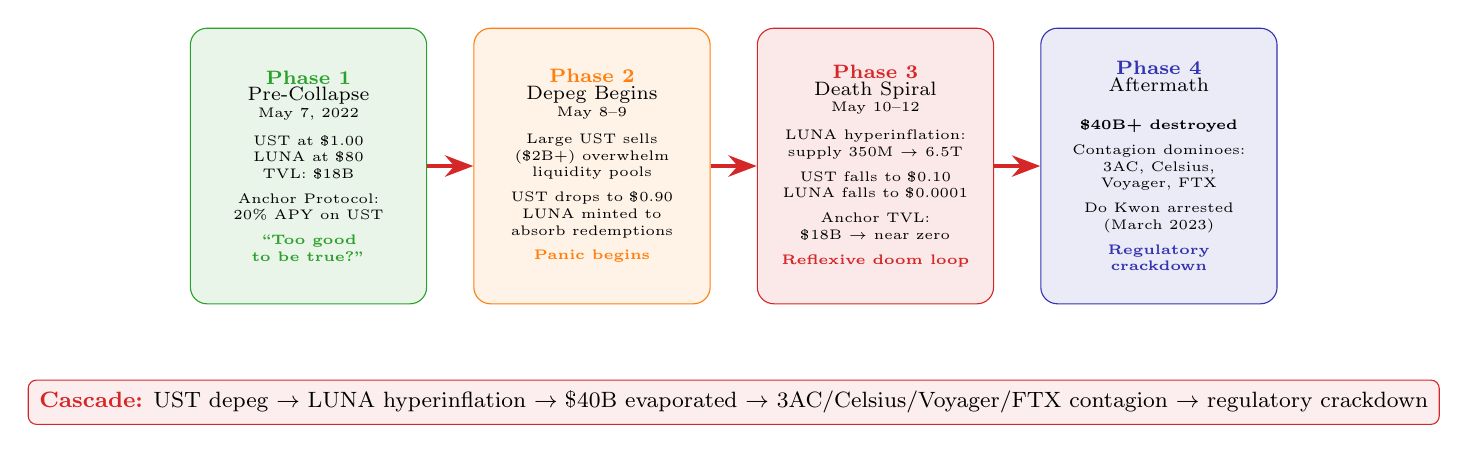
\begin{tikzpicture}[
  rwaphase/.style={draw,rounded corners=6pt,minimum width=3.0cm,minimum height=3.5cm,
    align=center,font=\tiny,inner sep=4pt},
  rwaphasearr/.style={-{Stealth},ultra thick}
]
  % Phase 1: Pre-collapse
  \node[rwaphase,fill=mlgreen!10,draw=mlgreen] (p1) at (0,0) {
    {\scriptsize\bfseries\color{mlgreen}Phase 1}\\
    {\scriptsize Pre-Collapse}\\
    {\tiny May 7, 2022}\\[4pt]
    UST at \$1.00\\
    LUNA at \$80\\
    TVL: \$18B\\[3pt]
    Anchor Protocol:\\
    20\% APY on UST\\[3pt]
    {\color{mlgreen}\textbf{``Too good}}\\
    {\color{mlgreen}\textbf{to be true?''}}};
  % Phase 2: Depeg begins
  \node[rwaphase,fill=mlorange!10,draw=mlorange] (p2) at (3.6,0) {
    {\scriptsize\bfseries\color{mlorange}Phase 2}\\
    {\scriptsize Depeg Begins}\\
    {\tiny May 8--9}\\[4pt]
    Large UST sells\\
    (\$2B+) overwhelm\\
    liquidity pools\\[3pt]
    UST drops to \$0.90\\
    LUNA minted to\\
    absorb redemptions\\[3pt]
    {\color{mlorange}\textbf{Panic begins}}};
  % Phase 3: Death spiral
  \node[rwaphase,fill=mlred!10,draw=mlred] (p3) at (7.2,0) {
    {\scriptsize\bfseries\color{mlred}Phase 3}\\
    {\scriptsize Death Spiral}\\
    {\tiny May 10--12}\\[4pt]
    LUNA hyperinflation:\\
    supply 350M $\rightarrow$ 6.5T\\[3pt]
    UST falls to \$0.10\\
    LUNA falls to \$0.0001\\[3pt]
    Anchor TVL:\\
    \$18B $\rightarrow$ near zero\\[3pt]
    {\color{mlred}\textbf{Reflexive doom loop}}};
  % Phase 4: Aftermath
  \node[rwaphase,fill=mlpurple!10,draw=mlpurple] (p4) at (10.8,0) {
    {\scriptsize\bfseries\color{mlpurple}Phase 4}\\
    {\scriptsize Aftermath}\\[8pt]
    \textbf{\$40B+ destroyed}\\[3pt]
    Contagion dominoes:\\
    3AC, Celsius,\\
    Voyager, FTX\\[3pt]
    Do Kwon arrested\\
    (March 2023)\\[3pt]
    {\color{mlpurple}\textbf{Regulatory}}\\
    {\color{mlpurple}\textbf{crackdown}}};
  % Red arrows between phases
  \draw[rwaphasearr,mlred] (p1.east) -- (p2.west);
  \draw[rwaphasearr,mlred] (p2.east) -- (p3.west);
  \draw[rwaphasearr,mlred] (p3.east) -- (p4.west);
  % Cascading loss annotation
  \node[draw=mlred,fill=mlred!8,rounded corners=3pt,minimum width=13.0cm,align=center,
    font=\footnotesize,inner sep=4pt] at (5.4,-3.0) {
    \textbf{\color{mlred}Cascade:} UST depeg $\rightarrow$ LUNA hyperinflation $\rightarrow$ \$40B evaporated $\rightarrow$
    3AC/Celsius/Voyager/FTX contagion $\rightarrow$ regulatory crackdown};
\end{tikzpicture}
\bottomnote{Terra/Luna was crypto's Lehman Brothers moment -- the death spiral proved that algorithmic stablecoins without real reserves are inherently fragile}
\end{frame}

% Frame 22: Stablecoin Reserve Models Compared
\begin{frame}{Stablecoin Reserve Models Compared}
\vspace{-2mm}
\begin{adjustbox}{max width=\textwidth}
\begin{tabular}{@{}l>{\scriptsize}c>{\scriptsize}c>{\scriptsize}c>{\scriptsize}c@{}}
\toprule
\textbf{\footnotesize Feature} & \textbf{USDT} & \textbf{USDC} & \textbf{DAI} & \textbf{PAXG} \\
\midrule
Type & Fiat-backed & Fiat-backed & Crypto-backed & Commodity-backed \\
\addlinespace
Market Cap & \$90B+ & \$30B+ & \$5B+ & \$500M+ \\
\addlinespace
Backing & T-bills/cash/loans & T-bills/cash & ETH/WBTC/RWA & Physical gold \\
\addlinespace
Collateral Ratio & 1:1 & 1:1 & 150\%+ & 1:1 \\
\addlinespace
Auditor & BDO Italia (quarterly) & Deloitte (monthly) & On-chain (real-time) & Withum (monthly) \\
\addlinespace
Depeg History & Brief depegs & SVB depeg \$0.87 & Brief MCD migration & None \\
\addlinespace
Regulation & Minimal & US regulated / MiCA & Decentralized & NYDFS regulated \\
\addlinespace
Chain Support & ETH/Tron/Solana & ETH/Solana/Base & Ethereum & Ethereum \\
\addlinespace
Risk Profile & Custodian + opacity & Banking system & Oracle + liquidation & Custodian \\
\bottomrule
\end{tabular}
\end{adjustbox}
\vspace{2mm}
\centering
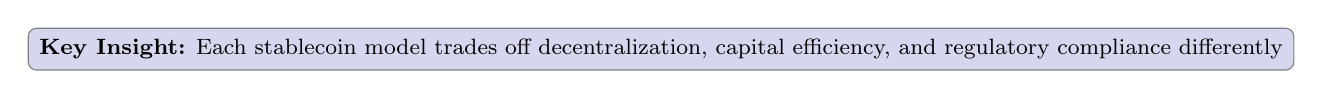
\begin{tikzpicture}
  \node[draw=mlgray,fill=mllavender4,rounded corners=3pt,minimum width=13.0cm,align=center,
    font=\footnotesize,inner sep=4pt] at (0,0) {
    \textbf{Key Insight:} Each stablecoin model trades off decentralization, capital efficiency, and regulatory compliance differently};
\end{tikzpicture}
\bottomnote{Each stablecoin model has a different risk profile -- there is no risk-free stablecoin, only different risk tradeoffs}
\end{frame}

% Frame 23: Stablecoin Market Dominance
\begin{frame}{Stablecoin Market Dominance}
\begin{columns}[T]
\column{0.52\textwidth}
\vspace{-2mm}
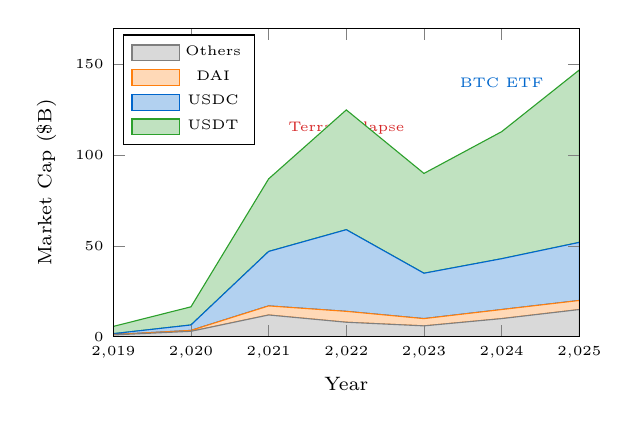
\begin{tikzpicture}
\begin{axis}[
  width=7.5cm, height=5.5cm,
  xlabel={Year},
  ylabel={Market Cap (\$B)},
  xmin=2019, xmax=2025,
  ymin=0, ymax=170,
  xtick={2019,2020,2021,2022,2023,2024,2025},
  xticklabel style={font=\tiny},
  yticklabel style={font=\tiny},
  xlabel style={font=\scriptsize},
  ylabel style={font=\scriptsize},
  legend style={font=\tiny,at={(0.02,0.98)},anchor=north west},
  area style,
  stack plots=y,
  enlarge x limits=false,
]
% Others (bottom layer)
\addplot[draw=mlgray,fill=mlgray!30] coordinates {
  (2019,1) (2020,3) (2021,12) (2022,8) (2023,6) (2024,10) (2025,15)
} \closedcycle;
\addlegendentry{Others}
% DAI
\addplot[draw=mlorange,fill=mlorange!30] coordinates {
  (2019,0.2) (2020,0.5) (2021,5) (2022,6) (2023,4) (2024,5) (2025,5)
} \closedcycle;
\addlegendentry{DAI}
% USDC
\addplot[draw=mlblue,fill=mlblue!30] coordinates {
  (2019,0.5) (2020,3) (2021,30) (2022,45) (2023,25) (2024,28) (2025,32)
} \closedcycle;
\addlegendentry{USDC}
% USDT (top layer)
\addplot[draw=mlgreen,fill=mlgreen!30] coordinates {
  (2019,4) (2020,10) (2021,40) (2022,66) (2023,55) (2024,70) (2025,95)
} \closedcycle;
\addlegendentry{USDT}
% Event annotations
\node[font=\tiny,mlpurple] at (axis cs:2020.5,2) {DeFi Summer};
\node[font=\tiny,mlred] at (axis cs:2022,115) {Terra collapse};
\node[font=\tiny,mlred] at (axis cs:2023,80) {SVB};
\node[font=\tiny,mlblue] at (axis cs:2024,140) {BTC ETF};
\end{axis}
\end{tikzpicture}

\column{0.44\textwidth}
\vspace{2mm}
\begin{block}{Key Statistics (2024/2025)}
\footnotesize
\begin{itemize}
  \item \textbf{Total market cap:} \$150B+
  \item \textbf{Daily settlement:} \$30--50B (rivaling traditional payment rails)
  \item \textbf{Annual on-chain:} \$10T+ (comparable to major card networks)
\end{itemize}
\end{block}
\vspace{2mm}
\begin{block}{Market Share}
\footnotesize
\begin{itemize}
  \item USDT: $\sim$60\%
  \item USDC: $\sim$20\%
  \item DAI: $\sim$3\%
  \item Others: $\sim$17\%
\end{itemize}
\end{block}
\vspace{2mm}
\begin{block}{Trend}
\footnotesize
USDT dominance grew during 2022--2023 bear market. USDC lost share after SVB depeg but recovering with MiCA compliance.
\end{block}
\end{columns}
\bottomnote{Stablecoins are the most successful blockchain use case by adoption -- settling trillions annually with growing institutional and retail usage}
\end{frame}

% Frame 24: Stablecoin Regulation
\begin{frame}{Stablecoin Regulation}
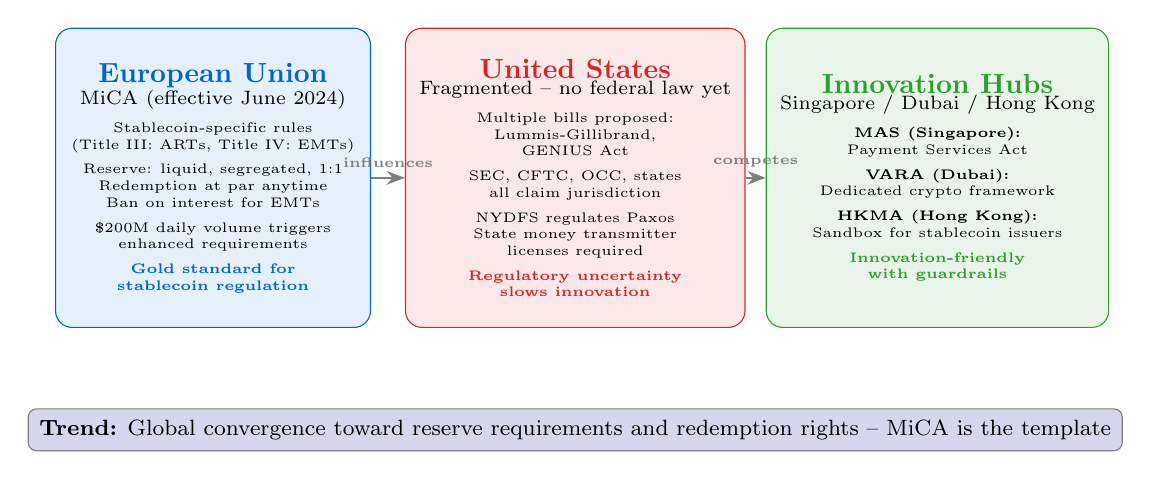
\begin{tikzpicture}[
  rwareg/.style={draw,rounded corners=6pt,minimum width=4.0cm,minimum height=3.8cm,
    align=center,font=\tiny,inner sep=5pt},
  rwaregarr/.style={-{Stealth},thick,mlgray}
]
  % EU (left)
  \node[rwareg,fill=mlblue!10,draw=mlblue] (eu) at (0,0) {
    {\normalsize\bfseries\color{mlblue}European Union}\\
    {\scriptsize MiCA (effective June 2024)}\\[4pt]
    Stablecoin-specific rules\\
    (Title III: ARTs, Title IV: EMTs)\\[3pt]
    Reserve: liquid, segregated, 1:1\\
    Redemption at par anytime\\
    Ban on interest for EMTs\\[3pt]
    \$200M daily volume triggers\\
    enhanced requirements\\[3pt]
    {\color{mlblue}\textbf{Gold standard for}}\\
    {\color{mlblue}\textbf{stablecoin regulation}}};
  % US (center)
  \node[rwareg,fill=mlred!10,draw=mlred] (us) at (4.6,0) {
    {\normalsize\bfseries\color{mlred}United States}\\
    {\scriptsize Fragmented -- no federal law yet}\\[4pt]
    Multiple bills proposed:\\
    Lummis-Gillibrand,\\
    GENIUS Act\\[3pt]
    SEC, CFTC, OCC, states\\
    all claim jurisdiction\\[3pt]
    NYDFS regulates Paxos\\
    State money transmitter\\
    licenses required\\[3pt]
    {\color{mlred}\textbf{Regulatory uncertainty}}\\
    {\color{mlred}\textbf{slows innovation}}};
  % Innovation hubs (right)
  \node[rwareg,fill=mlgreen!10,draw=mlgreen] (asia) at (9.2,0) {
    {\normalsize\bfseries\color{mlgreen}Innovation Hubs}\\
    {\scriptsize Singapore / Dubai / Hong Kong}\\[4pt]
    \textbf{MAS (Singapore):}\\
    Payment Services Act\\[3pt]
    \textbf{VARA (Dubai):}\\
    Dedicated crypto framework\\[3pt]
    \textbf{HKMA (Hong Kong):}\\
    Sandbox for stablecoin issuers\\[3pt]
    {\color{mlgreen}\textbf{Innovation-friendly}}\\
    {\color{mlgreen}\textbf{with guardrails}}};
  % Connecting arrows
  \draw[rwaregarr] (eu.east) -- node[above,font=\tiny\bfseries] {influences} (us.west);
  \draw[rwaregarr] (us.east) -- node[above,font=\tiny\bfseries] {competes} (asia.west);
  % Bottom annotation
  \node[draw=mlgray,fill=mllavender4,rounded corners=3pt,minimum width=13.0cm,align=center,
    font=\footnotesize,inner sep=4pt] at (4.6,-3.2) {
    \textbf{Trend:} Global convergence toward reserve requirements and redemption rights -- MiCA is the template};
\end{tikzpicture}
\bottomnote{MiCA is the world's first comprehensive crypto regulation -- its stablecoin rules set the global template for reserve and redemption requirements}
\end{frame}

% Frame 25: Section 2 Summary
\begin{frame}{Section 2 Summary: Stablecoins Deep Dive}
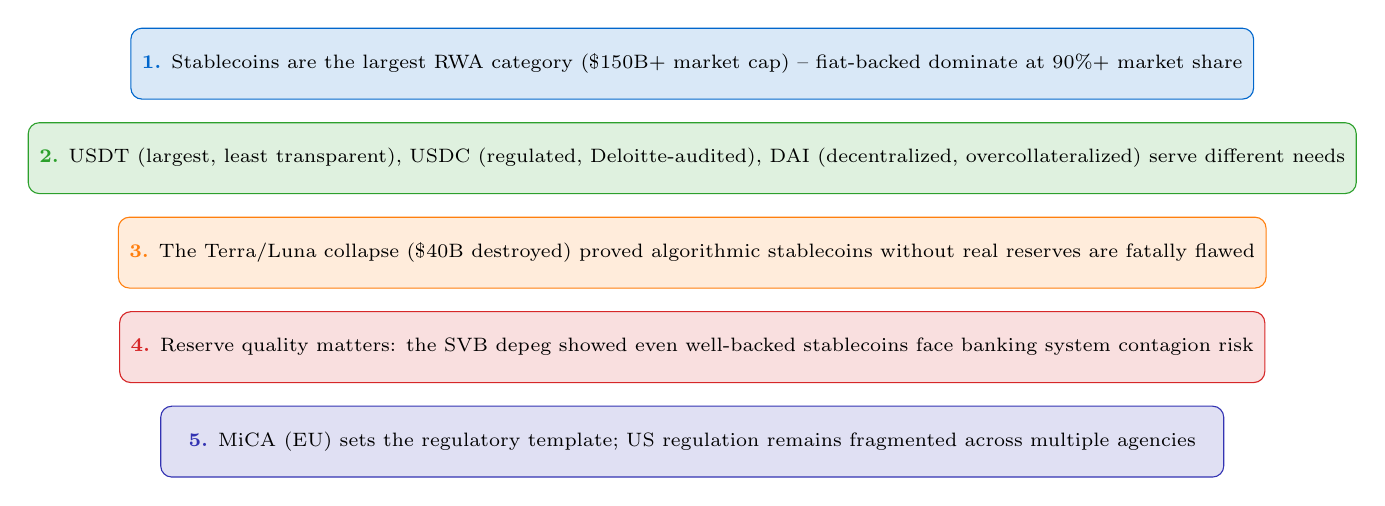
\begin{tikzpicture}[
  rwasummary/.style={draw,rounded corners=4pt,minimum width=13.5cm,minimum height=0.9cm,
    align=center,font=\scriptsize,inner sep=4pt}
]
  \node[rwasummary,fill=mlblue!15,draw=mlblue] at (6.5,2.0) {
    {\color{mlblue}\textbf{1.}} Stablecoins are the largest RWA category (\$150B+ market cap) -- fiat-backed dominate at 90\%+ market share};
  \node[rwasummary,fill=mlgreen!15,draw=mlgreen] at (6.5,0.8) {
    {\color{mlgreen}\textbf{2.}} USDT (largest, least transparent), USDC (regulated, Deloitte-audited), DAI (decentralized, overcollateralized) serve different needs};
  \node[rwasummary,fill=mlorange!15,draw=mlorange] at (6.5,-0.4) {
    {\color{mlorange}\textbf{3.}} The Terra/Luna collapse (\$40B destroyed) proved algorithmic stablecoins without real reserves are fatally flawed};
  \node[rwasummary,fill=mlred!15,draw=mlred] at (6.5,-1.6) {
    {\color{mlred}\textbf{4.}} Reserve quality matters: the SVB depeg showed even well-backed stablecoins face banking system contagion risk};
  \node[rwasummary,fill=mlpurple!15,draw=mlpurple] at (6.5,-2.8) {
    {\color{mlpurple}\textbf{5.}} MiCA (EU) sets the regulatory template; US regulation remains fragmented across multiple agencies};
\end{tikzpicture}
\bottomnote{Section 2 complete | Next: Section 3 -- Security Tokens \& Compliance}
\end{frame}

%% ============================================================
%% SECTION 3: SECURITY TOKENS & COMPLIANCE
%% ============================================================
\section{Security Tokens \& Compliance}

% Frame 26: Section 3 Divider
\begin{frame}{}
\begin{beamercolorbox}[sep=12pt,center,rounded=true,shadow=true]{palette quaternary}
  {\Large\bfseries Section 3: Security Tokens \& Compliance}\\[6pt]
  {\normalsize Legal classification, the Howey test, ERC-3643, and the regulated token economy}
\end{beamercolorbox}
\vspace{4mm}
\begin{columns}[T]
\column{0.5\textwidth}
\begin{block}{What You Will Learn}
\footnotesize
\begin{itemize}
  \item Security vs utility token classification and the Howey test
  \item SEC enforcement actions and regulatory precedents
  \item ERC-3643 (T-REX) standard for compliant security tokens
  \item Regulated exchanges, legal wrappers, and on-chain KYC/AML
\end{itemize}
\end{block}
\column{0.5\textwidth}
\begin{block}{Frames in This Section}
\footnotesize
\begin{itemize}
  \item Frame 27: Security vs Utility Tokens
  \item Frame 28: SEC Enforcement \& Precedents
  \item Frame 29: The Howey Test in Practice
  \item Frame 30: On-Chain KYC/AML Architecture
  \item Frame 31: ERC-3643 Compliant Transfer (Code)
  \item Frame 32: Transfer Restriction Patterns
  \item Frame 33: Regulated Security Token Exchanges
  \item Frame 34: Legal Wrappers for Tokenized Assets
  \item Frame 35: Tokenized vs Traditional Securities
  \item Frame 36: Section 3 Summary
\end{itemize}
\end{block}
\end{columns}
\bottomnote{Section 3 of 5 | Frames 26--36}
\end{frame}

% Frame 27: Security vs Utility Tokens
\begin{frame}{Security vs Utility Tokens}
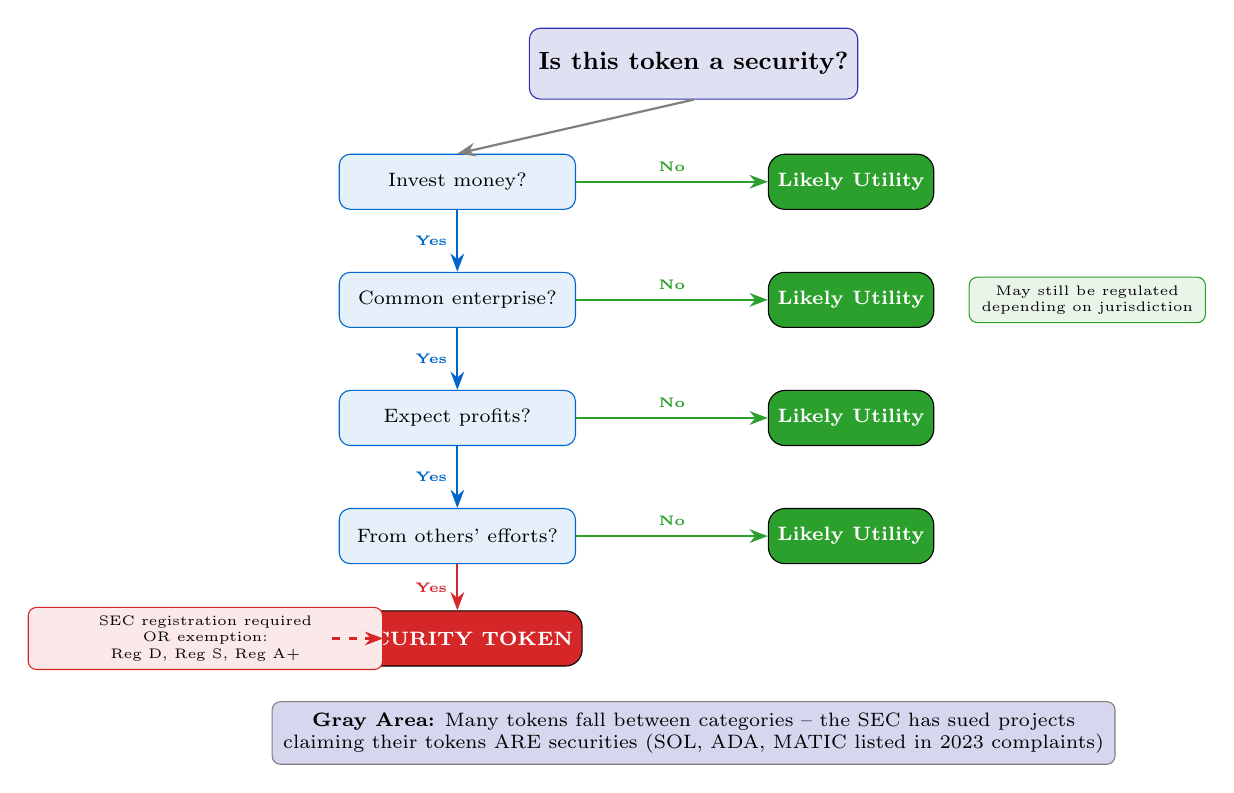
\begin{tikzpicture}[
  rwadecision/.style={draw,rounded corners=4pt,minimum width=3.0cm,minimum height=0.7cm,
    align=center,font=\scriptsize,fill=mlblue!10,draw=mlblue},
  rwayesno/.style={font=\tiny\bfseries},
  rwaresult/.style={draw,rounded corners=6pt,minimum width=2.4cm,minimum height=0.7cm,
    align=center,font=\scriptsize\bfseries,text=white},
  rwadecarr/.style={-{Stealth},thick,mlgray}
]
  % Root question
  \node[rwadecision,fill=mlpurple!15,draw=mlpurple,minimum width=4.0cm,minimum height=0.9cm,
    font=\small\bfseries] (root) at (6.5,3.5) {Is this token a security?};

  % Branch 1
  \node[rwadecision] (q1) at (3.5,2.0) {Invest money?};
  \node[rwadecision] (q2) at (3.5,0.5) {Common enterprise?};
  \node[rwadecision] (q3) at (3.5,-1.0) {Expect profits?};
  \node[rwadecision] (q4) at (3.5,-2.5) {From others' efforts?};

  % Security result
  \node[rwaresult,fill=mlred] (sec) at (3.5,-3.8) {SECURITY TOKEN};

  % Utility results
  \node[rwaresult,fill=mlgreen,minimum width=2.0cm] (u1) at (8.5,2.0) {Likely Utility};
  \node[rwaresult,fill=mlgreen,minimum width=2.0cm] (u2) at (8.5,0.5) {Likely Utility};
  \node[rwaresult,fill=mlgreen,minimum width=2.0cm] (u3) at (8.5,-1.0) {Likely Utility};
  \node[rwaresult,fill=mlgreen,minimum width=2.0cm] (u4) at (8.5,-2.5) {Likely Utility};

  % Arrows down (Yes path)
  \draw[rwadecarr] (root.south) -- (q1.north) node[midway,left,rwayesno] {};
  \draw[rwadecarr,mlblue] (q1.south) -- (q2.north) node[midway,left,rwayesno,mlblue] {Yes};
  \draw[rwadecarr,mlblue] (q2.south) -- (q3.north) node[midway,left,rwayesno,mlblue] {Yes};
  \draw[rwadecarr,mlblue] (q3.south) -- (q4.north) node[midway,left,rwayesno,mlblue] {Yes};
  \draw[rwadecarr,mlred] (q4.south) -- (sec.north) node[midway,left,rwayesno,mlred] {Yes};

  % Arrows right (No path)
  \draw[rwadecarr,mlgreen] (q1.east) -- (u1.west) node[midway,above,rwayesno,mlgreen] {No};
  \draw[rwadecarr,mlgreen] (q2.east) -- (u2.west) node[midway,above,rwayesno,mlgreen] {No};
  \draw[rwadecarr,mlgreen] (q3.east) -- (u3.west) node[midway,above,rwayesno,mlgreen] {No};
  \draw[rwadecarr,mlgreen] (q4.east) -- (u4.west) node[midway,above,rwayesno,mlgreen] {No};

  % Registration box
  \node[draw=mlred,fill=mlred!10,rounded corners=3pt,minimum width=4.5cm,align=center,
    font=\tiny,inner sep=3pt] (reg) at (0.3,-3.8) {SEC registration required\\OR exemption:\\Reg D, Reg S, Reg A+};
  \draw[rwadecarr,mlred,dashed] (sec.west) -- (reg.east);

  % Utility caveat
  \node[draw=mlgreen,fill=mlgreen!10,rounded corners=3pt,minimum width=3.0cm,align=center,
    font=\tiny,inner sep=3pt] at (11.5,0.5) {May still be regulated\\depending on jurisdiction};

  % Gray zone callout
  \node[draw=mlgray,fill=mllavender4,rounded corners=3pt,minimum width=7.5cm,align=center,
    font=\scriptsize,inner sep=4pt] at (6.5,-5.0) {
    \textbf{Gray Area:} Many tokens fall between categories -- the SEC has sued projects\\
    claiming their tokens ARE securities (SOL, ADA, MATIC listed in 2023 complaints)};
\end{tikzpicture}
\bottomnote{The Howey test dates from 1946 (SEC v.\ W.J.\ Howey Co.) -- it was designed for orange grove investments but now determines crypto classification}
\end{frame}

% Frame 28: SEC Enforcement & Precedents
\begin{frame}{SEC Enforcement \& Precedents}
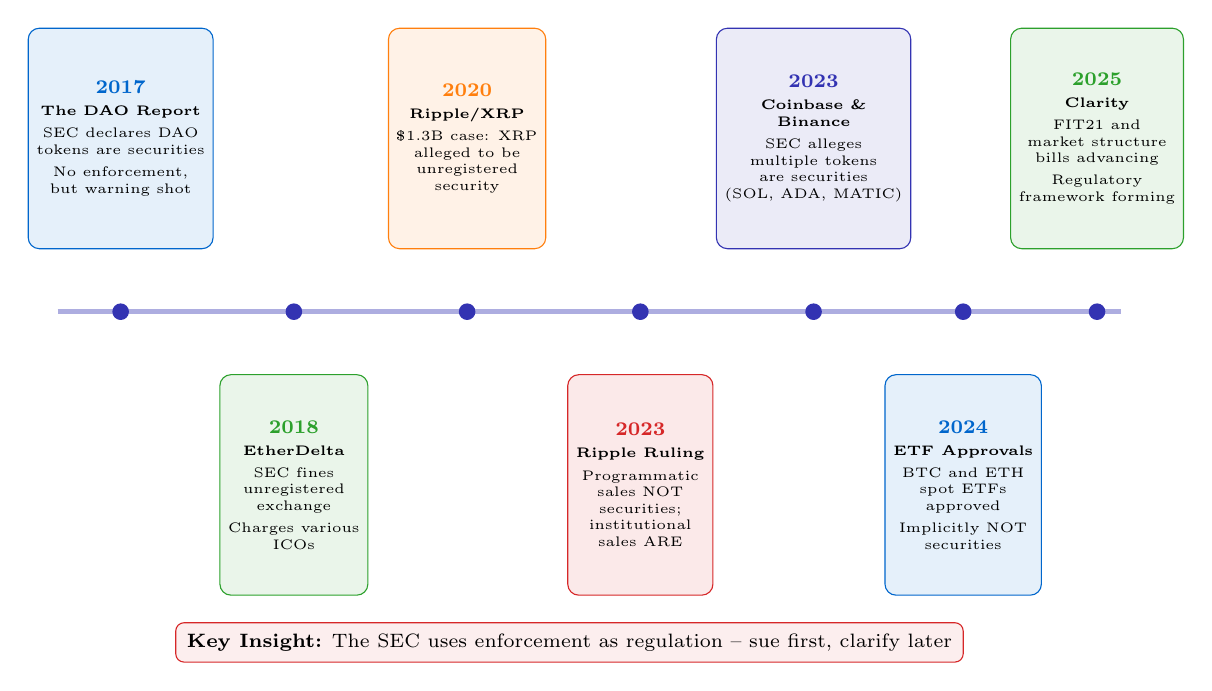
\begin{tikzpicture}[
  rwacase/.style={draw,rounded corners=4pt,minimum width=1.5cm,minimum height=2.8cm,
    align=center,font=\tiny,inner sep=3pt},
  rwacasearr/.style={-{Stealth},thick,mlgray},
  rwacasedot/.style={circle,fill=mlpurple,minimum size=6pt,inner sep=0pt}
]
  % Timeline line
  \draw[ultra thick,mllavender] (0,0) -- (13.5,0);

  % 2017
  \node[rwacasedot] (d1) at (0.8,0) {};
  \node[rwacase,fill=mlblue!10,draw=mlblue] at (0.8,2.2) {
    {\scriptsize\bfseries\color{mlblue}2017}\\[2pt]
    \textbf{The DAO Report}\\[2pt]
    SEC declares DAO\\
    tokens are securities\\[2pt]
    No enforcement,\\
    but warning shot};

  % 2018
  \node[rwacasedot] (d2) at (3.0,0) {};
  \node[rwacase,fill=mlgreen!10,draw=mlgreen] at (3.0,-2.2) {
    {\scriptsize\bfseries\color{mlgreen}2018}\\[2pt]
    \textbf{EtherDelta}\\[2pt]
    SEC fines\\
    unregistered\\
    exchange\\[2pt]
    Charges various\\
    ICOs};

  % 2020
  \node[rwacasedot] (d3) at (5.2,0) {};
  \node[rwacase,fill=mlorange!10,draw=mlorange] at (5.2,2.2) {
    {\scriptsize\bfseries\color{mlorange}2020}\\[2pt]
    \textbf{Ripple/XRP}\\[2pt]
    \$1.3B case: XRP\\
    alleged to be\\
    unregistered\\
    security};

  % 2023a
  \node[rwacasedot] (d4) at (7.4,0) {};
  \node[rwacase,fill=mlred!10,draw=mlred] at (7.4,-2.2) {
    {\scriptsize\bfseries\color{mlred}2023}\\[2pt]
    \textbf{Ripple Ruling}\\[2pt]
    Programmatic\\
    sales NOT\\
    securities;\\
    institutional\\
    sales ARE};

  % 2023b
  \node[rwacasedot] (d5) at (9.6,0) {};
  \node[rwacase,fill=mlpurple!10,draw=mlpurple] at (9.6,2.2) {
    {\scriptsize\bfseries\color{mlpurple}2023}\\[2pt]
    \textbf{Coinbase \&}\\
    \textbf{Binance}\\[2pt]
    SEC alleges\\
    multiple tokens\\
    are securities\\
    (SOL, ADA, MATIC)};

  % 2024
  \node[rwacasedot] (d6) at (11.5,0) {};
  \node[rwacase,fill=mlblue!10,draw=mlblue] at (11.5,-2.2) {
    {\scriptsize\bfseries\color{mlblue}2024}\\[2pt]
    \textbf{ETF Approvals}\\[2pt]
    BTC and ETH\\
    spot ETFs\\
    approved\\[2pt]
    Implicitly NOT\\
    securities};

  % 2025
  \node[rwacasedot] (d7) at (13.2,0) {};
  \node[rwacase,fill=mlgreen!10,draw=mlgreen] at (13.2,2.2) {
    {\scriptsize\bfseries\color{mlgreen}2025}\\[2pt]
    \textbf{Clarity}\\[2pt]
    FIT21 and\\
    market structure\\
    bills advancing\\[2pt]
    Regulatory\\
    framework forming};

  % Key insight
  \node[draw=mlred,fill=mlred!8,rounded corners=3pt,minimum width=8.0cm,align=center,
    font=\scriptsize,inner sep=4pt] at (6.5,-4.2) {
    \textbf{Key Insight:} The SEC uses enforcement as regulation -- sue first, clarify later};
\end{tikzpicture}
\bottomnote{The Ripple ruling created a split: programmatic exchange sales may not be securities, but direct institutional sales are -- a nuanced precedent}
\end{frame}

% Frame 29: The Howey Test in Practice
\begin{frame}{The Howey Test in Practice}
\begin{columns}[T]
\column{0.44\textwidth}
\begin{block}{\color{mlred}Passes Howey Test (IS a Security)}
\footnotesize
\begin{itemize}
  \item Token sale funding a project development team
  \item Tokens with profit-sharing from company revenue
  \item Tokens whose value depends on management team efforts
  \item Tokenized real estate with rental yield
  \item Tokenized equity or debt instruments
\end{itemize}
\vspace{2mm}
\scriptsize
\textbf{Examples:} Many 2017 ICO tokens, LBRY Credits (SEC won)
\end{block}

\column{0.44\textwidth}
\begin{block}{\color{mlgreen}Fails Howey Test (NOT a Security)}
\footnotesize
\begin{itemize}
  \item Decentralized network tokens where no single party drives value
  \item Utility tokens providing access to a live, functioning product
  \item Governance tokens with no profit expectation (debatable)
  \item Sufficiently decentralized tokens (the ``Hinman test'' -- Ethereum)
  \item Bitcoin (commodity per CFTC)
\end{itemize}
\vspace{2mm}
\scriptsize
\textbf{Examples:} BTC, ETH (per SEC guidance)
\end{block}
\end{columns}

\vspace{3mm}
\begin{center}
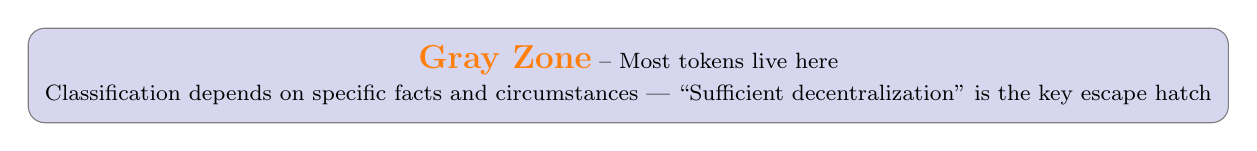
\begin{tikzpicture}
  \node[draw=mlgray,fill=mllavender4,rounded corners=6pt,minimum width=12.0cm,
    minimum height=1.2cm,align=center,font=\footnotesize,inner sep=6pt] {
    {\large\bfseries\color{mlorange}Gray Zone} -- Most tokens live here\\[2pt]
    Classification depends on specific facts and circumstances | ``Sufficient decentralization'' is the key escape hatch};
\end{tikzpicture}
\end{center}
\bottomnote{The distinction often comes down to ``sufficient decentralization'' -- if no single entity drives the token's value, it may escape security classification}
\end{frame}

% Frame 30: On-Chain KYC/AML Architecture
\begin{frame}{On-Chain KYC/AML Architecture}
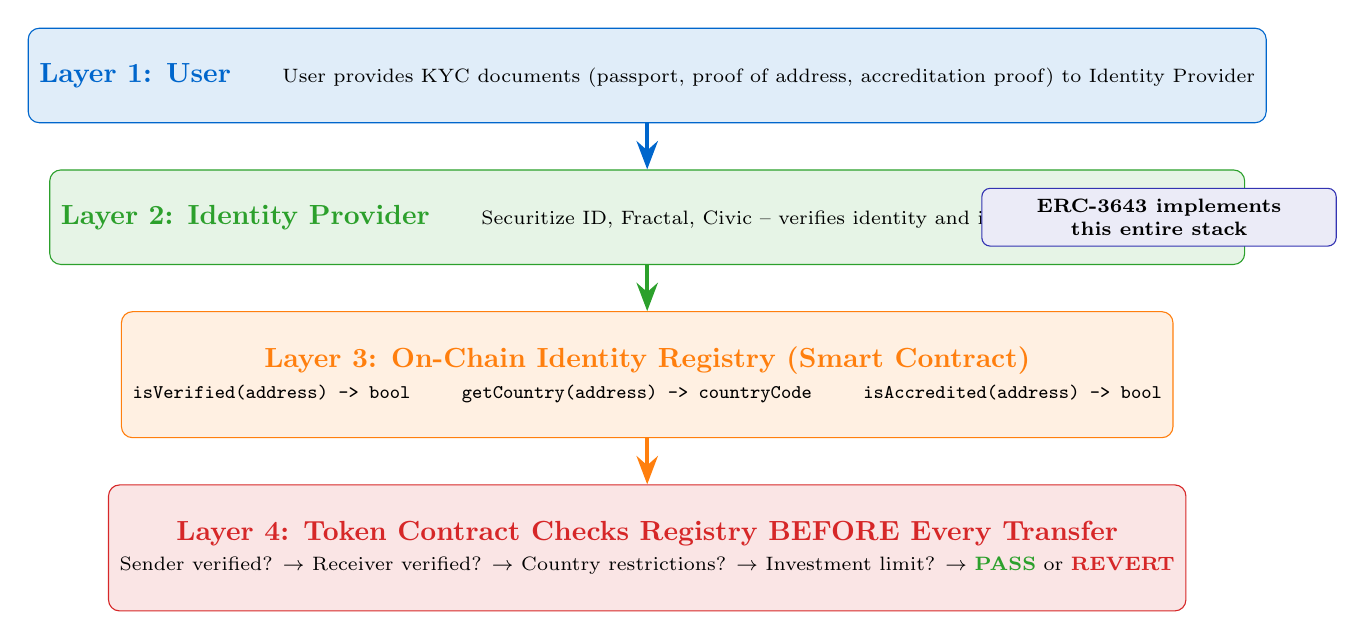
\begin{tikzpicture}[
  rwalayer/.style={draw,rounded corners=4pt,minimum height=1.2cm,
    align=center,font=\scriptsize,inner sep=4pt},
  rwalayerarr/.style={-{Stealth},ultra thick,mlgray}
]
  % Layer 1: User
  \node[rwalayer,fill=mlblue!12,draw=mlblue,minimum width=13.0cm] (l1) at (6.5,3.0) {
    {\normalsize\bfseries\color{mlblue}Layer 1: User}
    \quad\quad User provides KYC documents (passport, proof of address, accreditation proof) to Identity Provider};

  % Layer 2: Identity Provider
  \node[rwalayer,fill=mlgreen!12,draw=mlgreen,minimum width=13.0cm] (l2) at (6.5,1.2) {
    {\normalsize\bfseries\color{mlgreen}Layer 2: Identity Provider}
    \quad\quad Securitize ID, Fractal, Civic -- verifies identity and issues on-chain attestation};

  % Layer 3: On-chain Registry
  \node[rwalayer,fill=mlorange!12,draw=mlorange,minimum width=13.0cm,minimum height=1.6cm] (l3) at (6.5,-0.8) {
    {\normalsize\bfseries\color{mlorange}Layer 3: On-Chain Identity Registry (Smart Contract)}\\[3pt]
    \texttt{isVerified(address) -> bool} \quad\quad
    \texttt{getCountry(address) -> countryCode} \quad\quad
    \texttt{isAccredited(address) -> bool}};

  % Layer 4: Token Contract
  \node[rwalayer,fill=mlred!12,draw=mlred,minimum width=13.0cm,minimum height=1.6cm] (l4) at (6.5,-3.0) {
    {\normalsize\bfseries\color{mlred}Layer 4: Token Contract Checks Registry BEFORE Every Transfer}\\[3pt]
    Sender verified? $\rightarrow$ Receiver verified? $\rightarrow$ Country restrictions? $\rightarrow$ Investment limit?
    $\rightarrow$ {\color{mlgreen}\textbf{PASS}} or {\color{mlred}\textbf{REVERT}}};

  % Arrows between layers
  \draw[rwalayerarr,mlblue] (l1.south) -- (l2.north);
  \draw[rwalayerarr,mlgreen] (l2.south) -- (l3.north);
  \draw[rwalayerarr,mlorange] (l3.south) -- (l4.north);

  % ERC-3643 annotation
  \node[draw=mlpurple,fill=mlpurple!10,rounded corners=3pt,minimum width=4.5cm,align=center,
    font=\scriptsize\bfseries,inner sep=4pt] at (13.0,1.2) {ERC-3643 implements\\this entire stack};
\end{tikzpicture}
\bottomnote{On-chain KYC turns compliance from a manual process into programmable logic -- every transfer is automatically checked against compliance rules}
\end{frame}

% Frame 31: ERC-3643 Compliant Transfer [CODE FRAME 3]
\begin{frame}[fragile]{ERC-3643 Compliant Transfer}
\begin{columns}[T]
\column{0.48\textwidth}
\begin{lstlisting}
// Simplified ERC-3643 Token
contract SecurityToken {
    IIdentityRegistry public
        identityRegistry;
    ICompliance public compliance;

    mapping(address => uint256)
        public balanceOf;

    function transfer(
        address to,
        uint256 amount
    ) external returns (bool) {
        require(
            identityRegistry
                .isVerified(msg.sender),
            "Sender not verified"
        );
        require(
            identityRegistry
                .isVerified(to),
            "Receiver not verified"
        );
        require(
            compliance.canTransfer(
                msg.sender, to, amount
            ),
            "Compliance check failed"
        );
        balanceOf[msg.sender] -= amount;
        balanceOf[to] += amount;
        return true;
    }
}
\end{lstlisting}

\column{0.48\textwidth}
\vspace{2mm}
\begin{block}{Identity Registry Checks}
\footnotesize
\begin{itemize}
  \item \textbf{isVerified()}: Checks both sender and receiver have completed KYC through an approved Identity Provider
  \item On-chain attestation links wallet address to verified identity claim
  \item Identity can be revoked if KYC expires or sanctions list changes
\end{itemize}
\end{block}
\vspace{2mm}
\begin{block}{Compliance Module}
\footnotesize
\begin{itemize}
  \item \textbf{canTransfer()}: Enforces country restrictions, investor limits, lockup periods, and volume caps
  \item Modular: swap compliance rules without redeploying the token contract
  \item Issuer configures rules per jurisdiction
\end{itemize}
\end{block}
\vspace{2mm}
\begin{block}{ERC-3643 in Production}
\footnotesize
\begin{itemize}
  \item Wraps ERC-20 with a compliance layer -- all standard ERC-20 functions still work
  \item Developed by Tokeny Solutions -- 500+ deployments on Ethereum and Polygon
  \item Also known as T-REX (Token for Regulated EXchanges)
\end{itemize}
\end{block}
\end{columns}
\bottomnote{ERC-3643 is the most widely adopted security token standard -- it adds identity and compliance checks to the familiar ERC-20 interface}
\end{frame}

% Frame 32: Transfer Restriction Patterns
\begin{frame}{Transfer Restriction Patterns}
\begin{tikzpicture}[
  rwapanel/.style={draw,rounded corners=4pt,minimum width=4.2cm,minimum height=2.6cm,
    align=center,font=\tiny,inner sep=4pt}
]
  % Row 1
  \node[rwapanel,fill=mlblue!10,draw=mlblue] at (0,1.5) {
    {\scriptsize\bfseries\color{mlblue}Country Restrictions}\\[4pt]
    Block transfers to/from\\sanctioned countries (OFAC list)\\[3pt]
    \begin{tikzpicture}[scale=0.35]
      \node[circle,fill=mlblue!30,minimum size=12mm] (globe) {};
      \node[font=\tiny\bfseries] at (globe) {WORLD};
      \node[circle,fill=mlred,minimum size=3mm,font=\tiny\bfseries,text=white] at (0.5,0.4) {X};
      \node[circle,fill=mlred,minimum size=3mm,font=\tiny\bfseries,text=white] at (-0.4,-0.3) {X};
    \end{tikzpicture}};

  \node[rwapanel,fill=mlgreen!10,draw=mlgreen] at (4.6,1.5) {
    {\scriptsize\bfseries\color{mlgreen}Investor Limits}\\[4pt]
    Max token holders\\(Reg D 506(c): accredited only,\\max 2000 before SEC reporting)\\[3pt]
    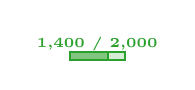
\begin{tikzpicture}[scale=0.35]
      \draw[thick,mlgreen,fill=mlgreen!20] (0,0) rectangle (2.0,0.3);
      \draw[thick,mlgreen,fill=mlgreen!60] (0,0) rectangle (1.4,0.3);
      \node[font=\tiny\bfseries,mlgreen] at (1.0,0.6) {1,400 / 2,000};
    \end{tikzpicture}};

  \node[rwapanel,fill=mlorange!10,draw=mlorange] at (9.2,1.5) {
    {\scriptsize\bfseries\color{mlorange}Lockup Periods}\\[4pt]
    Tokens locked for X months\\after issuance (vesting)\\[3pt]
    
\begin{tikzpicture}[scale=0.35]
      \draw[thick,mlorange] (0,0) -- (3,0);
      \node[circle,fill=mlred,minimum size=3mm,inner sep=0pt] at (0,0) {};
      \node[circle,fill=mlorange,minimum size=3mm,inner sep=0pt] at (1.5,0) {};
      \node[circle,fill=mlgreen,minimum size=3mm,inner sep=0pt] at (3,0) {};
      \node[font=\tiny] at (0,-0.5) {Issue};
      \node[font=\tiny] at (1.5,-0.5) {6mo};
      \node[font=\tiny] at (3,-0.5) {Unlock};
    \end{tikzpicture}};

  % Row 2
  \node[rwapanel,fill=mlred!10,draw=mlred] at (0,-1.7) {
    {\scriptsize\bfseries\color{mlred}Transfer Volume Limits}\\[4pt]
    Max transfer size per period\\(anti-money laundering)\\[3pt]
    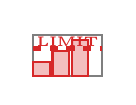
\begin{tikzpicture}[scale=0.35]
      \draw[thick,mlgray] (0,0) rectangle (2.5,1.5);
      \draw[thick,mlred,fill=mlred!30] (0,0) rectangle (0.6,0.5);
      \draw[thick,mlred,fill=mlred!30] (0.7,0) rectangle (1.3,0.9);
      \draw[thick,mlred,fill=mlred!30] (1.4,0) rectangle (2.0,1.3);
      \draw[ultra thick,mlred,dashed] (0,1.0) -- (2.5,1.0);
      \node[font=\tiny\bfseries,mlred] at (1.25,1.25) {LIMIT};
    \end{tikzpicture}};

  \node[rwapanel,fill=mlpurple!10,draw=mlpurple] at (4.6,-1.7) {
    {\scriptsize\bfseries\color{mlpurple}Accreditation Check}\\[4pt]
    Only accredited investors\\(\$1M+ net worth or\\
    \$200K+ annual income)\\[3pt]
    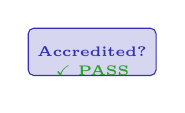
\begin{tikzpicture}[scale=0.35]
      \node[draw,mlpurple,rounded corners=2pt,minimum width=1.5cm,minimum height=0.6cm,
        fill=mlpurple!20,font=\tiny\bfseries] {Accredited?};
      \node[font=\tiny\bfseries,mlgreen] at (0,-0.7) {$\checkmark$ PASS};
    \end{tikzpicture}};

  \node[rwapanel,fill=mlgray!15,draw=mlgray] at (9.2,-1.7) {
    {\scriptsize\bfseries\color{mlgray}Forced Transfer}\\[4pt]
    Issuer can forcibly transfer\\tokens (court order, regulatory\\action, lost keys recovery)\\[3pt]
    
\begin{tikzpicture}[scale=0.35]
      \draw[-{Stealth},ultra thick,mlred] (0,0) -- (2,0);
      \node[circle,fill=mlgray,minimum size=4mm,inner sep=0pt,font=\tiny\bfseries,text=white] at (1,0.5) {!};
      \node[font=\tiny] at (1,-0.5) {Override};
    \end{tikzpicture}};
\end{tikzpicture}
\bottomnote{These restrictions exist in traditional securities too -- tokenization makes them programmable and automatic rather than manual and error-prone}
\end{frame}

% Frame 33: Regulated Security Token Exchanges
\begin{frame}{Regulated Security Token Exchanges}
\begin{columns}[T]
\column{0.48\textwidth}
\begin{block}{Exchange Landscape}
\footnotesize
\begin{itemize}
  \item \textbf{tZERO} (US): Overstock-backed, SEC-registered ATS. Trades tokenized equity, real estate, digital securities
  \item \textbf{Securitize Markets} (US): SEC-registered broker-dealer and ATS. Largest platform by issuances (500+). End-to-end: issuance + compliance + trading
  \item \textbf{INX} (Israel/US): SEC-registered security token exchange. First SEC-registered IPO on blockchain
  \item \textbf{SIX Digital Exchange} (Switzerland): FINMA-regulated. First fully regulated digital asset exchange by traditional exchange operator
  \item \textbf{Archax} (UK): FCA-regulated. Focused on institutional investors
\end{itemize}
\end{block}

\column{0.48\textwidth}
\vspace{2mm}
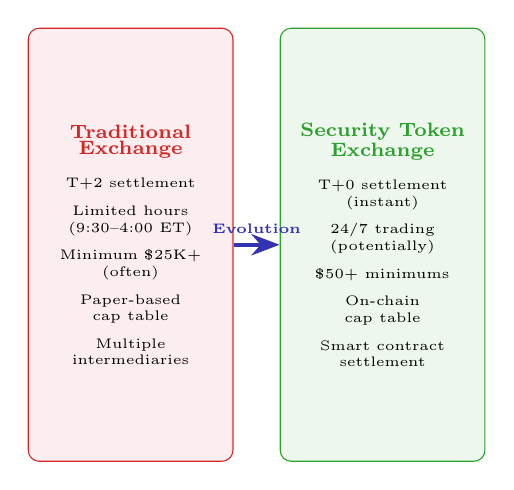
\begin{tikzpicture}[
  rwaexcol/.style={draw,rounded corners=4pt,minimum width=2.6cm,minimum height=5.5cm,
    align=center,font=\tiny,inner sep=4pt}
]
  % Traditional
  \node[rwaexcol,fill=mlred!8,draw=mlred] (trad) at (0,0) {
    {\scriptsize\bfseries\color{mlred}Traditional}\\
    {\scriptsize\bfseries\color{mlred}Exchange}\\[6pt]
    T+2 settlement\\[4pt]
    Limited hours\\(9:30--4:00 ET)\\[4pt]
    Minimum \$25K+\\(often)\\[4pt]
    Paper-based\\cap table\\[4pt]
    Multiple\\intermediaries};

  % Security Token
  \node[rwaexcol,fill=mlgreen!8,draw=mlgreen] (sto) at (3.2,0) {
    {\scriptsize\bfseries\color{mlgreen}Security Token}\\
    {\scriptsize\bfseries\color{mlgreen}Exchange}\\[6pt]
    T+0 settlement\\(instant)\\[4pt]
    24/7 trading\\(potentially)\\[4pt]
    \$50+ minimums\\[4pt]
    On-chain\\cap table\\[4pt]
    Smart contract\\settlement};

  % Arrow between
  \draw[-{Stealth},ultra thick,mlpurple] (trad.east) -- (sto.west)
    node[midway,above,font=\tiny\bfseries,mlpurple] {Evolution};
\end{tikzpicture}
\end{columns}
\bottomnote{The security token exchange landscape is still early -- combined daily volume across all STO exchanges is tiny compared to traditional exchanges}
\end{frame}

% Frame 34: Legal Wrappers for Tokenized Assets
\begin{frame}{Legal Wrappers for Tokenized Assets}
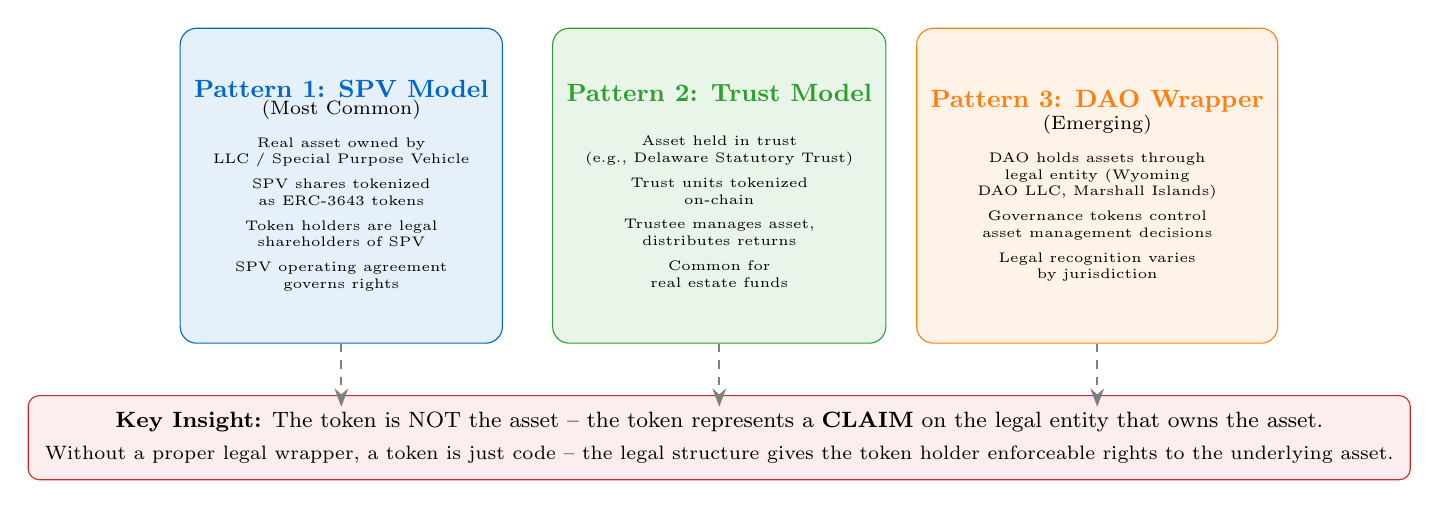
\begin{tikzpicture}[
  rwawrap/.style={draw,rounded corners=6pt,minimum width=4.0cm,minimum height=4.0cm,
    align=center,font=\tiny,inner sep=5pt},
  rwawraparr/.style={-{Stealth},thick,mlgray}
]
  % Pattern 1: SPV Model
  \node[rwawrap,fill=mlblue!10,draw=mlblue] (spv) at (0,0) {
    {\small\bfseries\color{mlblue}Pattern 1: SPV Model}\\
    {\scriptsize (Most Common)}\\[6pt]
    Real asset owned by\\LLC / Special Purpose Vehicle\\[3pt]
    SPV shares tokenized\\as ERC-3643 tokens\\[3pt]
    Token holders are legal\\shareholders of SPV\\[3pt]
    SPV operating agreement\\governs rights};

  % Pattern 2: Trust Model
  \node[rwawrap,fill=mlgreen!10,draw=mlgreen] (trust) at (4.8,0) {
    {\small\bfseries\color{mlgreen}Pattern 2: Trust Model}\\[10pt]
    Asset held in trust\\(e.g., Delaware Statutory Trust)\\[3pt]
    Trust units tokenized\\on-chain\\[3pt]
    Trustee manages asset,\\distributes returns\\[3pt]
    Common for\\real estate funds};

  % Pattern 3: DAO Wrapper
  \node[rwawrap,fill=mlorange!10,draw=mlorange] (dao) at (9.6,0) {
    {\small\bfseries\color{mlorange}Pattern 3: DAO Wrapper}\\
    {\scriptsize (Emerging)}\\[6pt]
    DAO holds assets through\\legal entity (Wyoming\\DAO LLC, Marshall Islands)\\[3pt]
    Governance tokens control\\asset management decisions\\[3pt]
    Legal recognition varies\\by jurisdiction};

  % Key insight
  \node[draw=mlred,fill=mlred!8,rounded corners=4pt,minimum width=13.0cm,align=center,
    font=\footnotesize,inner sep=6pt] at (4.8,-3.2) {
    \textbf{Key Insight:} The token is NOT the asset -- the token represents a \textbf{CLAIM}
    on the legal entity that owns the asset.\\[2pt]
    {\scriptsize Without a proper legal wrapper, a token is just code --
    the legal structure gives the token holder enforceable rights to the underlying asset.}};

  % Arrows from patterns to insight
  \draw[rwawraparr,dashed] (spv.south) -- ++(0,-0.8);
  \draw[rwawraparr,dashed] (trust.south) -- ++(0,-0.8);
  \draw[rwawraparr,dashed] (dao.south) -- ++(0,-0.8);
\end{tikzpicture}
\bottomnote{Without a proper legal wrapper, a token is just code -- the legal structure is what gives the token holder enforceable rights to the underlying asset}
\end{frame}

% Frame 35: Tokenized vs Traditional Securities
\begin{frame}{Tokenized vs Traditional Securities}
\vspace{-2mm}
\begin{adjustbox}{max width=\textwidth}
\begin{tabular}{@{}l l l@{}}
\toprule
\textbf{Dimension} & \textbf{Traditional Securities} & \textbf{Tokenized Securities} \\
\midrule
Settlement Time & T+2 days & T+0 (instant on-chain) \\
Trading Hours & 9:30--4:00 M--F & 24/7 (potentially) \\
Minimum Investment & Often \$10K+ & \$50+ \\
Custody & Custodian bank required & Self-custody or institutional wallet \\
Dividend Distribution & Wire transfer (5--10 business days) & Smart contract (instant) \\
Cap Table & Paper / spreadsheet & On-chain (real-time, auditable) \\
Compliance & Manual (lawyers, transfer agents) & Automated (ERC-3643) \\
Cross-Border Access & Complex (different depositories) & Native (blockchain is global) \\
Issuance Cost & \$500K--\$5M & \$50K--\$500K \\
Secondary Liquidity & Established exchanges & Early-stage exchanges \\
Investor Eligibility & Accredited + retail (post-IPO) & Mostly accredited (for now) \\
Regulatory Status & Well-established & Evolving \\
\bottomrule
\end{tabular}
\end{adjustbox}
\vspace{3mm}
\begin{center}
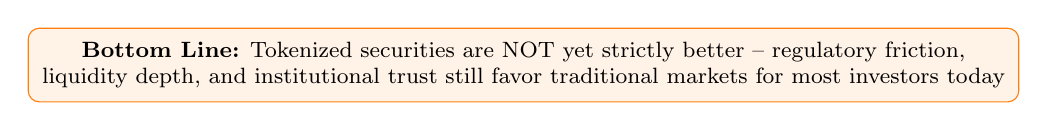
\begin{tikzpicture}
  \node[draw=mlorange,fill=mlorange!10,rounded corners=4pt,minimum width=12.0cm,
    align=center,font=\footnotesize,inner sep=5pt] {
    \textbf{Bottom Line:} Tokenized securities are NOT yet strictly better -- regulatory friction,\\
    liquidity depth, and institutional trust still favor traditional markets for most investors today};
\end{tikzpicture}
\end{center}
\bottomnote{Tokenized securities are NOT yet strictly better -- regulatory friction, liquidity, and institutional trust still favor traditional markets for most investors}
\end{frame}

% Frame 36: Section 3 Summary
\begin{frame}{Section 3 Summary: Security Tokens \& Compliance}
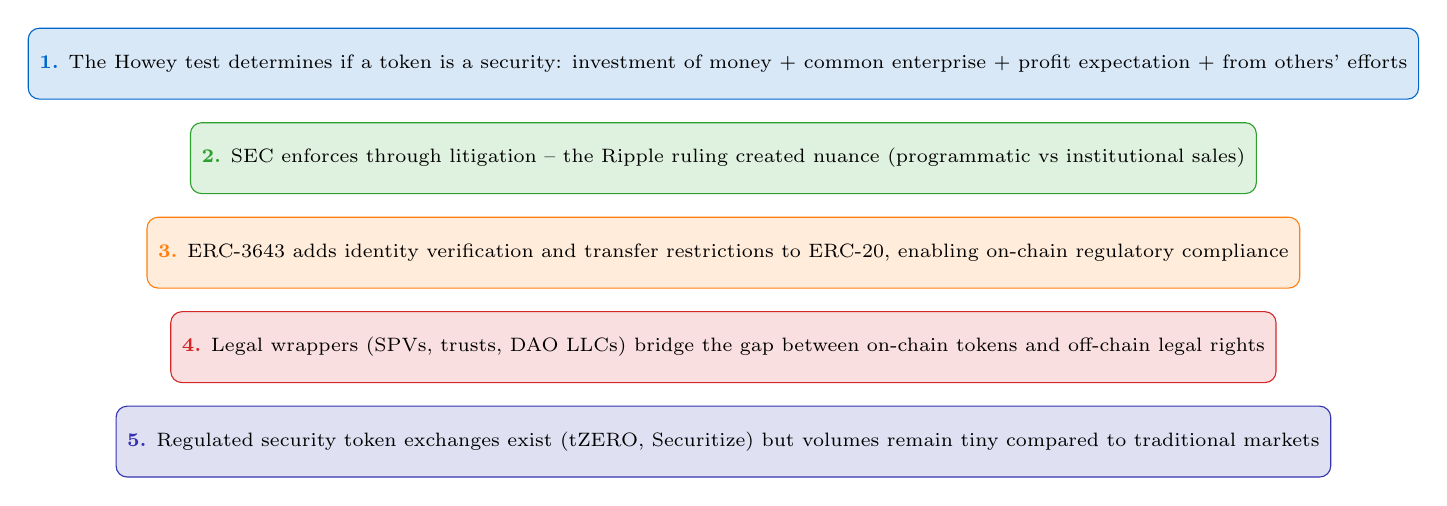
\begin{tikzpicture}[
  rwasummary/.style={draw,rounded corners=4pt,minimum width=13.5cm,minimum height=0.9cm,
    align=center,font=\scriptsize,inner sep=4pt}
]
  \node[rwasummary,fill=mlblue!15,draw=mlblue] at (6.5,2.0) {
    {\color{mlblue}\textbf{1.}} The Howey test determines if a token is a security: investment of money + common enterprise + profit expectation + from others' efforts};
  \node[rwasummary,fill=mlgreen!15,draw=mlgreen] at (6.5,0.8) {
    {\color{mlgreen}\textbf{2.}} SEC enforces through litigation -- the Ripple ruling created nuance (programmatic vs institutional sales)};
  \node[rwasummary,fill=mlorange!15,draw=mlorange] at (6.5,-0.4) {
    {\color{mlorange}\textbf{3.}} ERC-3643 adds identity verification and transfer restrictions to ERC-20, enabling on-chain regulatory compliance};
  \node[rwasummary,fill=mlred!15,draw=mlred] at (6.5,-1.6) {
    {\color{mlred}\textbf{4.}} Legal wrappers (SPVs, trusts, DAO LLCs) bridge the gap between on-chain tokens and off-chain legal rights};
  \node[rwasummary,fill=mlpurple!15,draw=mlpurple] at (6.5,-2.8) {
    {\color{mlpurple}\textbf{5.}} Regulated security token exchanges exist (tZERO, Securitize) but volumes remain tiny compared to traditional markets};
\end{tikzpicture}
\bottomnote{Section 3 complete | Next: Section 4 -- Tokenized Treasuries \& Institutional DeFi}
\end{frame}

%% ============================================================
%% SECTION 4: REAL ESTATE & BOND TOKENIZATION
%% ============================================================
\section{Real Estate \& Bond Tokenization}

% Frame 37: Section 4 Divider
\begin{frame}{}
\begin{beamercolorbox}[sep=12pt,center,rounded=true,shadow=true]{palette quaternary}
  {\Large\bfseries Section 4: Real Estate \& Bond Tokenization}\\[6pt]
  {\normalsize Platforms, institutional adoption, yield-bearing tokens, and real-world case studies}
\end{beamercolorbox}
\vspace{4mm}
\begin{columns}[T]
\column{0.5\textwidth}
\begin{block}{What You Will Learn}
\footnotesize
\begin{itemize}
  \item Real estate tokenization mechanics and platforms (RealT, Centrifuge)
  \item Bond tokenization by institutions (JPMorgan, Siemens, EIB)
  \item Private credit markets on-chain (Maple Finance, Goldfinch)
  \item Yield-bearing tokens: tokenized T-bills and institutional products
\end{itemize}
\end{block}
\column{0.5\textwidth}
\begin{block}{Frames in This Section}
\footnotesize
\begin{itemize}
  \item Frame 38: Real Estate Tokenization Architecture
  \item Frame 39: RealT Platform Deep Dive
  \item Frame 40: Centrifuge Protocol
  \item Frame 41: Maple Finance \& On-Chain Credit
  \item Frame 42: Bond Tokenization Case Studies
  \item Frame 43: Yield-Bearing Token Contract (Code)
  \item Frame 44: Yield-Bearing Token Landscape
  \item Frame 45: Institutional Adoption Drivers
  \item Frame 46: Private Credit On-Chain
  \item Frame 47: Section 4 Summary
\end{itemize}
\end{block}
\end{columns}
\bottomnote{Section 4 covers real estate, bonds, private credit, and yield-bearing tokens -- the fastest-growing RWA categories}
\end{frame}

% Frame 38: Real Estate Tokenization Architecture
\begin{frame}{Real Estate Tokenization Architecture}
\vspace{-2mm}
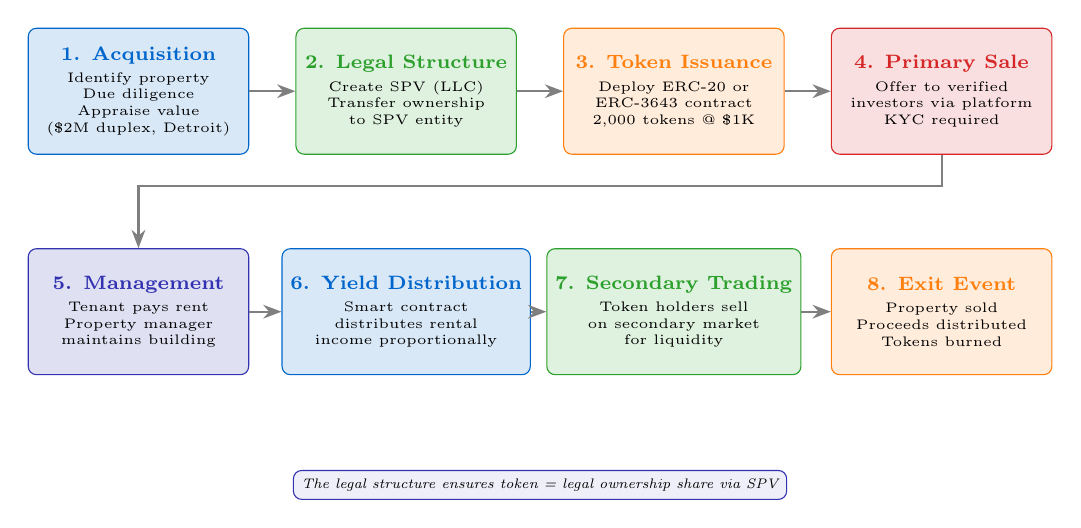
\begin{tikzpicture}[
  rwastep/.style={draw,rounded corners=3pt,minimum width=2.8cm,minimum height=1.6cm,
    align=center,font=\tiny,inner sep=3pt},
  rwaarrow/.style={-{Stealth},thick,mlgray}
]
  % Row 1: Steps 1-4
  \node[rwastep,fill=mlblue!15,draw=mlblue] (s1) at (0,0) {
    {\color{mlblue}\scriptsize\textbf{1. Acquisition}}\\[2pt]
    Identify property\\Due diligence\\Appraise value\\(\$2M duplex, Detroit)};
  \node[rwastep,fill=mlgreen!15,draw=mlgreen] (s2) at (3.4,0) {
    {\color{mlgreen}\scriptsize\textbf{2. Legal Structure}}\\[2pt]
    Create SPV (LLC)\\Transfer ownership\\to SPV entity};
  \node[rwastep,fill=mlorange!15,draw=mlorange] (s3) at (6.8,0) {
    {\color{mlorange}\scriptsize\textbf{3. Token Issuance}}\\[2pt]
    Deploy ERC-20 or\\ERC-3643 contract\\2{,}000 tokens @ \$1K};
  \node[rwastep,fill=mlred!15,draw=mlred] (s4) at (10.2,0) {
    {\color{mlred}\scriptsize\textbf{4. Primary Sale}}\\[2pt]
    Offer to verified\\investors via platform\\KYC required};
  % Row 2: Steps 5-8
  \node[rwastep,fill=mlpurple!15,draw=mlpurple] (s5) at (0,-2.8) {
    {\color{mlpurple}\scriptsize\textbf{5. Management}}\\[2pt]
    Tenant pays rent\\Property manager\\maintains building};
  \node[rwastep,fill=mlblue!15,draw=mlblue] (s6) at (3.4,-2.8) {
    {\color{mlblue}\scriptsize\textbf{6. Yield Distribution}}\\[2pt]
    Smart contract\\distributes rental\\income proportionally};
  \node[rwastep,fill=mlgreen!15,draw=mlgreen] (s7) at (6.8,-2.8) {
    {\color{mlgreen}\scriptsize\textbf{7. Secondary Trading}}\\[2pt]
    Token holders sell\\on secondary market\\for liquidity};
  \node[rwastep,fill=mlorange!15,draw=mlorange] (s8) at (10.2,-2.8) {
    {\color{mlorange}\scriptsize\textbf{8. Exit Event}}\\[2pt]
    Property sold\\Proceeds distributed\\Tokens burned};
  % Arrows row 1
  \draw[rwaarrow] (s1.east) -- (s2.west);
  \draw[rwaarrow] (s2.east) -- (s3.west);
  \draw[rwaarrow] (s3.east) -- (s4.west);
  % Arrow down from row 1 to row 2
  \draw[rwaarrow] (s4.south) -- ++(0,-0.4) -| (s5.north);
  % Arrows row 2
  \draw[rwaarrow] (s5.east) -- (s6.west);
  \draw[rwaarrow] (s6.east) -- (s7.west);
  \draw[rwaarrow] (s7.east) -- (s8.west);
  % Annotation
  \node[draw=mlpurple,fill=mlpurple!8,rounded corners=3pt,font=\tiny\itshape,inner sep=3pt]
    at (5.1,-5.0) {The legal structure ensures token = legal ownership share via SPV};
\end{tikzpicture}
\bottomnote{Real estate tokenization combines PropTech, DeFi, and securities law -- each step requires expertise in legal, technical, and regulatory domains}
\end{frame}

% Frame 39: RealT Platform Deep Dive
\begin{frame}{RealT Platform Deep Dive}
\begin{columns}[T]
\column{0.52\textwidth}
\vspace{2mm}
\footnotesize
\begin{block}{RealT Overview}
\begin{itemize}
  \item Pioneer in real estate tokenization (launched 2019)
  \item Properties: US residential (Detroit, Chicago, Cleveland)
  \item Blockchain: Gnosis Chain (low fees, fast transactions)
  \item Token standard: ERC-20 (each property = separate token)
  \item Minimum investment: \textasciitilde\$50 per token
  \item Rental yield: distributed weekly in USDC via smart contract
  \item Average yield: 8--12\% APY (rental income)
  \item Portfolio: 500+ properties tokenized
  \item DeFi integration: RealT tokens as collateral on RMM (RealT Money Market)
\end{itemize}
\end{block}

\column{0.46\textwidth}
\vspace{2mm}
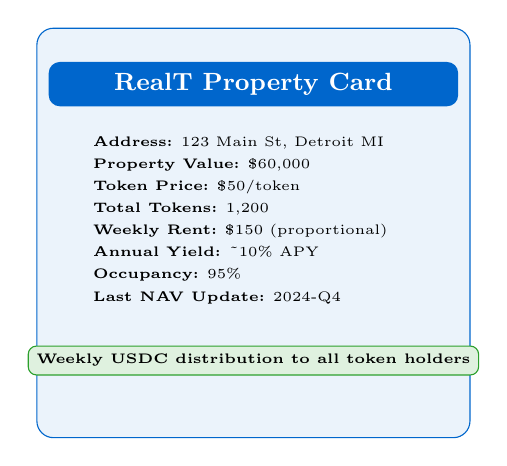
\begin{tikzpicture}[scale=0.9]
  % Property card
  \node[draw=mlblue,fill=mlblue!8,rounded corners=6pt,minimum width=5.5cm,
    minimum height=5.2cm,inner sep=0pt] (card) at (0,0) {};
  % Header
  \node[fill=mlblue,text=white,rounded corners=4pt,minimum width=5.2cm,
    font=\small\bfseries,inner sep=4pt] at (0,2.1) {RealT Property Card};
  % Details
  \node[font=\tiny,align=left,anchor=north west] at (-2.4,1.5) {
    \textbf{Address:} 123 Main St, Detroit MI\\[2pt]
    \textbf{Property Value:} \$60{,}000\\[2pt]
    \textbf{Token Price:} \$50/token\\[2pt]
    \textbf{Total Tokens:} 1{,}200\\[2pt]
    \textbf{Weekly Rent:} \$150 (proportional)\\[2pt]
    \textbf{Annual Yield:} \textasciitilde10\% APY\\[2pt]
    \textbf{Occupancy:} 95\%\\[2pt]
    \textbf{Last NAV Update:} 2024-Q4
  };
  % Yield highlight
  \node[draw=mlgreen,fill=mlgreen!15,rounded corners=3pt,font=\tiny\bfseries,inner sep=3pt]
    at (0,-1.8) {Weekly USDC distribution to all token holders};
\end{tikzpicture}
\end{columns}
\bottomnote{RealT is the largest tokenized real estate platform by number of properties -- 500+ US residential properties available to global investors for \$50+}
\end{frame}

% Frame 40: Centrifuge Protocol
\begin{frame}{Centrifuge Protocol}
\begin{columns}[T]
\column{0.50\textwidth}
\vspace{2mm}
\footnotesize
\begin{block}{Centrifuge Architecture}
\begin{itemize}
  \item Tokenizes real-world credit (not just real estate):
    \begin{itemize}\tiny
      \item Trade finance invoices
      \item Revenue-based financing
      \item US Treasury bills
      \item Mortgage-backed loans
      \item Warehouse credit lines
    \end{itemize}
  \item Centrifuge Chain: Substrate-based (bridges to Ethereum)
  \item Pool structure: Senior + Junior tranches
  \item Tinlake: DeFi lending protocol for Centrifuge assets
  \item MakerDAO integration: \$200M+ RWA collateral
  \item TVL: \$300M+
\end{itemize}
\end{block}

\column{0.48\textwidth}
\vspace{2mm}
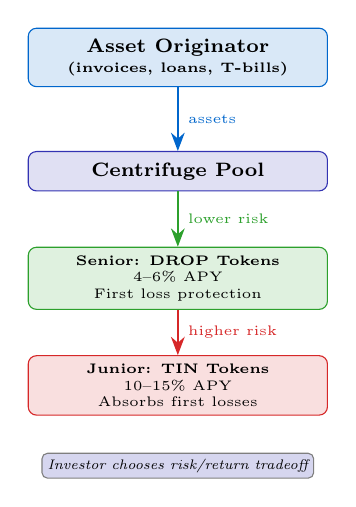
\begin{tikzpicture}[scale=0.85]
  % Asset originator
  \node[draw=mlblue,fill=mlblue!15,rounded corners=3pt,minimum width=3.8cm,
    font=\scriptsize\bfseries,align=center,inner sep=4pt] (orig) at (0,2.5)
    {Asset Originator\\[-1pt]\tiny (invoices, loans, T-bills)};
  % Pool
  \node[draw=mlpurple,fill=mlpurple!15,rounded corners=3pt,minimum width=3.8cm,
    font=\scriptsize\bfseries,inner sep=4pt,align=center] (pool) at (0,0.8)
    {Centrifuge Pool};
  % Senior tranche
  \node[draw=mlgreen,fill=mlgreen!15,rounded corners=3pt,minimum width=3.8cm,
    font=\tiny,align=center,inner sep=3pt] (senior) at (0,-0.8)
    {\textbf{Senior: DROP Tokens}\\4--6\% APY\\First loss protection};
  % Junior tranche
  \node[draw=mlred,fill=mlred!15,rounded corners=3pt,minimum width=3.8cm,
    font=\tiny,align=center,inner sep=3pt] (junior) at (0,-2.4)
    {\textbf{Junior: TIN Tokens}\\10--15\% APY\\Absorbs first losses};
  % Arrows
  \draw[-{Stealth},thick,mlblue] (orig) -- node[right,font=\tiny]{assets} (pool);
  \draw[-{Stealth},thick,mlgreen] (pool) -- node[right,font=\tiny]{lower risk} (senior);
  \draw[-{Stealth},thick,mlred] (senior) -- node[right,font=\tiny]{higher risk} (junior);
  % Investor annotation
  \node[draw=mlgray,fill=mllavender4,rounded corners=2pt,font=\tiny\itshape,inner sep=2pt]
    at (0,-3.6) {Investor chooses risk/return tradeoff};
\end{tikzpicture}
\end{columns}
\bottomnote{Centrifuge pioneered structured credit on-chain -- tranching allows different risk appetites, exactly like traditional asset-backed securities}
\end{frame}

% Frame 41: Maple Finance & On-Chain Credit
\begin{frame}{Maple Finance \& On-Chain Credit}
\begin{columns}[T]
\column{0.50\textwidth}
\vspace{2mm}
\footnotesize
\begin{block}{Maple Finance}
\begin{itemize}
  \item Institutional undercollateralized lending on-chain
  \item Pool delegates (credit experts) assess borrower creditworthiness
  \item Borrowers: crypto market makers, trading firms, fintech companies
  \item Lending: USDC or wETH, fixed-term loans
  \item History: launched 2021, \$2B+ total lending volume
  \item Post-2022 crisis: bad debts from Alameda Research, Orthogonal Trading defaults
  \item Recovery: pivoted to institutional-grade underwriting, over-collateralized pools
  \item Maple Direct: compliant lending to institutions
\end{itemize}
\end{block}

\column{0.48\textwidth}
\vspace{2mm}
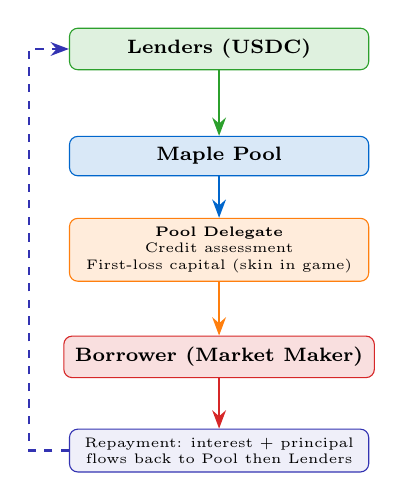
\begin{tikzpicture}[scale=0.85]
  % Lenders
  \node[draw=mlgreen,fill=mlgreen!15,rounded corners=3pt,minimum width=3.8cm,
    font=\scriptsize\bfseries,align=center,inner sep=4pt] (lenders) at (0,2.8)
    {Lenders (USDC)};
  % Pool
  \node[draw=mlblue,fill=mlblue!15,rounded corners=3pt,minimum width=3.8cm,
    font=\scriptsize\bfseries,align=center,inner sep=4pt] (mpool) at (0,1.2)
    {Maple Pool};
  % Pool delegate
  \node[draw=mlorange,fill=mlorange!15,rounded corners=3pt,minimum width=3.8cm,
    font=\tiny,align=center,inner sep=3pt] (delegate) at (0,-0.2)
    {\textbf{Pool Delegate}\\Credit assessment\\First-loss capital (skin in game)};
  % Borrower
  \node[draw=mlred,fill=mlred!15,rounded corners=3pt,minimum width=3.8cm,
    font=\scriptsize\bfseries,align=center,inner sep=4pt] (borrower) at (0,-1.8)
    {Borrower (Market Maker)};
  % Repayment
  \node[draw=mlpurple,fill=mlpurple!8,rounded corners=3pt,minimum width=3.8cm,
    font=\tiny,align=center,inner sep=3pt] (repay) at (0,-3.2)
    {Repayment: interest + principal\\flows back to Pool then Lenders};
  % Arrows
  \draw[-{Stealth},thick,mlgreen] (lenders) -- (mpool);
  \draw[-{Stealth},thick,mlblue] (mpool) -- (delegate);
  \draw[-{Stealth},thick,mlorange] (delegate) -- (borrower);
  \draw[-{Stealth},thick,mlred] (borrower) -- (repay);
  \draw[-{Stealth},thick,dashed,mlpurple] (repay.west) -- ++(-0.6,0) |- (lenders.west);
\end{tikzpicture}
\end{columns}
\bottomnote{Maple's 2022 defaults (\$50M+) showed that undercollateralized on-chain lending carries real credit risk -- just like traditional banking}
\end{frame}

% Frame 42: Bond Tokenization Case Studies
\begin{frame}{Bond Tokenization Case Studies}
\vspace{-2mm}
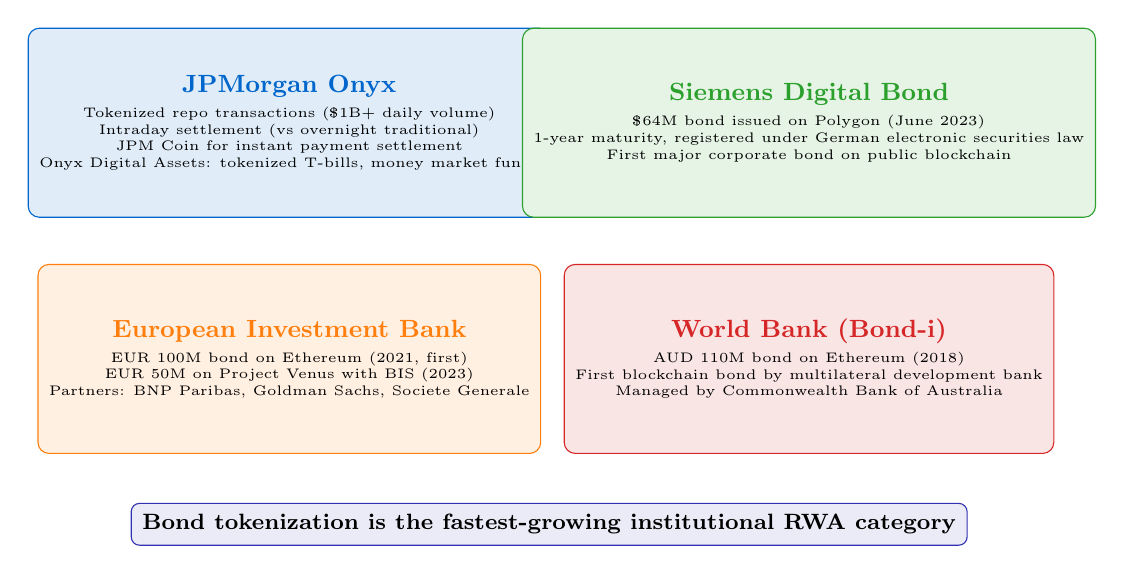
\begin{tikzpicture}[
  rwacase/.style={draw,rounded corners=4pt,minimum width=5.8cm,minimum height=2.4cm,
    align=center,font=\tiny,inner sep=4pt}
]
  % Case 1: JPMorgan
  \node[rwacase,fill=mlblue!12,draw=mlblue] (c1) at (3.2,1.5) {
    {\color{mlblue}\small\textbf{JPMorgan Onyx}}\\[3pt]
    Tokenized repo transactions (\$1B+ daily volume)\\
    Intraday settlement (vs overnight traditional)\\
    JPM Coin for instant payment settlement\\
    Onyx Digital Assets: tokenized T-bills, money market funds};
  % Case 2: Siemens
  \node[rwacase,fill=mlgreen!12,draw=mlgreen] (c2) at (9.8,1.5) {
    {\color{mlgreen}\small\textbf{Siemens Digital Bond}}\\[3pt]
    \$64M bond issued on Polygon (June 2023)\\
    1-year maturity, registered under German electronic securities law\\
    First major corporate bond on public blockchain};
  % Case 3: EIB
  \node[rwacase,fill=mlorange!12,draw=mlorange] (c3) at (3.2,-1.5) {
    {\color{mlorange}\small\textbf{European Investment Bank}}\\[3pt]
    EUR 100M bond on Ethereum (2021, first)\\
    EUR 50M on Project Venus with BIS (2023)\\
    Partners: BNP Paribas, Goldman Sachs, Societe Generale};
  % Case 4: World Bank
  \node[rwacase,fill=mlred!12,draw=mlred] (c4) at (9.8,-1.5) {
    {\color{mlred}\small\textbf{World Bank (Bond-i)}}\\[3pt]
    AUD 110M bond on Ethereum (2018)\\
    First blockchain bond by multilateral development bank\\
    Managed by Commonwealth Bank of Australia};
  % Central label
  \node[draw=mlpurple,fill=mlpurple!10,rounded corners=3pt,font=\footnotesize\bfseries,inner sep=4pt]
    at (6.5,-3.6) {Bond tokenization is the fastest-growing institutional RWA category};
\end{tikzpicture}
\bottomnote{Bond tokenization savings come from instant settlement, 24/7 operations, and automated coupon payments}
\end{frame}

% Frame 43: Yield-Bearing Token Contract [CODE FRAME 4]
\begin{frame}[fragile]{Yield-Bearing Token (Tokenized T-Bill)}
\begin{columns}[T]
\column{0.48\textwidth}
\begin{lstlisting}
// Simplified Yield-Bearing Token
contract TokenizedTBill {
    string public name =
        "Tokenized US T-Bill";
    uint256 public totalShares;
    uint256 public totalAssets;

    mapping(address => uint256)
        public shares;

    function deposit(
        uint256 usdcAmount
    ) external {
        uint256 newShares =
            totalAssets == 0
            ? usdcAmount
            : usdcAmount
              * totalShares
              / totalAssets;
        shares[msg.sender] += newShares;
        totalShares += newShares;
        totalAssets += usdcAmount;
        // Transfer USDC from user
    }

    function rebase(
        uint256 yieldAmount
    ) external onlyManager {
        totalAssets += yieldAmount;
        // Share price increases
    }
}
\end{lstlisting}
\column{0.50\textwidth}
\vspace{2mm}
\begin{block}{Rebasing Vault Pattern (ERC-4626)}
\footnotesize
\begin{itemize}
  \item Vault holds underlying assets (T-bills via custodian)
  \item Users deposit USDC, receive \textbf{shares}
  \item Share price = \texttt{totalAssets / totalShares}
  \item Manager calls \texttt{rebase()} as T-bills earn interest
  \item \texttt{totalAssets} increases $\Rightarrow$ share price rises
  \item No token transfer needed -- value accrues automatically
\end{itemize}
\end{block}
\vspace{2mm}
\begin{block}{Real-World Examples}
\footnotesize
\begin{itemize}
  \item \textbf{Ondo USDY:} 5.2\% APY (T-bills + bank deposits)
  \item \textbf{Franklin BENJI:} 5.0\% APY (US Gov Money Fund)
  \item \textbf{MakerDAO sDAI:} 5--8\% APY (variable, DSR)
  \item All use variants of this rebasing/vault pattern
\end{itemize}
\end{block}
\end{columns}
\bottomnote{The ERC-4626 vault standard is becoming the de facto pattern for yield-bearing tokens -- deposit assets, receive shares, value accrues via rebase}
\end{frame}

% Frame 44: Yield-Bearing Token Landscape
\begin{frame}{Yield-Bearing Token Landscape}
\vspace{-2mm}
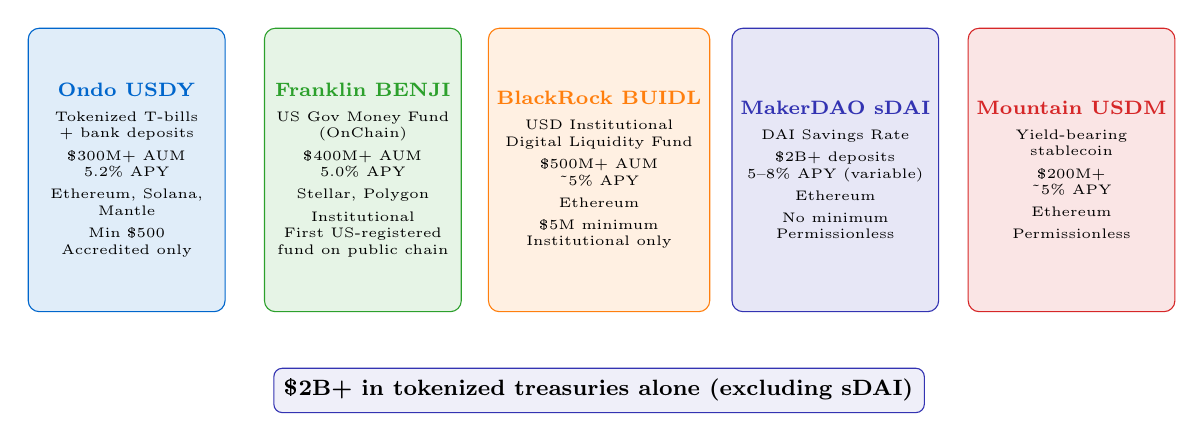
\begin{tikzpicture}[
  rwaprod/.style={draw,rounded corners=4pt,minimum width=2.5cm,minimum height=3.6cm,
    align=center,font=\tiny,inner sep=3pt}
]
  % Ondo USDY
  \node[rwaprod,fill=mlblue!12,draw=mlblue] (p1) at (0,0) {
    {\color{mlblue}\scriptsize\textbf{Ondo USDY}}\\[3pt]
    Tokenized T-bills\\+ bank deposits\\[2pt]
    \$300M+ AUM\\5.2\% APY\\[2pt]
    Ethereum, Solana,\\Mantle\\[2pt]
    Min \$500\\Accredited only};
  % Franklin BENJI
  \node[rwaprod,fill=mlgreen!12,draw=mlgreen] (p2) at (3.0,0) {
    {\color{mlgreen}\scriptsize\textbf{Franklin BENJI}}\\[3pt]
    US Gov Money Fund\\(OnChain)\\[2pt]
    \$400M+ AUM\\5.0\% APY\\[2pt]
    Stellar, Polygon\\[2pt]
    Institutional\\First US-registered\\fund on public chain};
  % BlackRock BUIDL
  \node[rwaprod,fill=mlorange!12,draw=mlorange] (p3) at (6.0,0) {
    {\color{mlorange}\scriptsize\textbf{BlackRock BUIDL}}\\[3pt]
    USD Institutional\\Digital Liquidity Fund\\[2pt]
    \$500M+ AUM\\\textasciitilde5\% APY\\[2pt]
    Ethereum\\[2pt]
    \$5M minimum\\Institutional only};
  % MakerDAO sDAI
  \node[rwaprod,fill=mlpurple!12,draw=mlpurple] (p4) at (9.0,0) {
    {\color{mlpurple}\scriptsize\textbf{MakerDAO sDAI}}\\[3pt]
    DAI Savings Rate\\[2pt]
    \$2B+ deposits\\5--8\% APY (variable)\\[2pt]
    Ethereum\\[2pt]
    No minimum\\Permissionless};
  % Mountain USDM
  \node[rwaprod,fill=mlred!12,draw=mlred] (p5) at (12.0,0) {
    {\color{mlred}\scriptsize\textbf{Mountain USDM}}\\[3pt]
    Yield-bearing\\stablecoin\\[2pt]
    \$200M+\\\textasciitilde5\% APY\\[2pt]
    Ethereum\\[2pt]
    Permissionless};
  % Key stat
  \node[draw=mlpurple,fill=mlpurple!8,rounded corners=3pt,font=\footnotesize\bfseries,inner sep=4pt]
    at (6.0,-2.8) {\$2B+ in tokenized treasuries alone (excluding sDAI)};
\end{tikzpicture}
\bottomnote{Yield-bearing tokens brought the ``risk-free rate'' on-chain -- DeFi users can now earn Treasury yields without leaving the blockchain ecosystem}
\end{frame}

% Frame 45: Institutional Adoption Drivers
\begin{frame}{Institutional Adoption Drivers}
\vspace{-2mm}
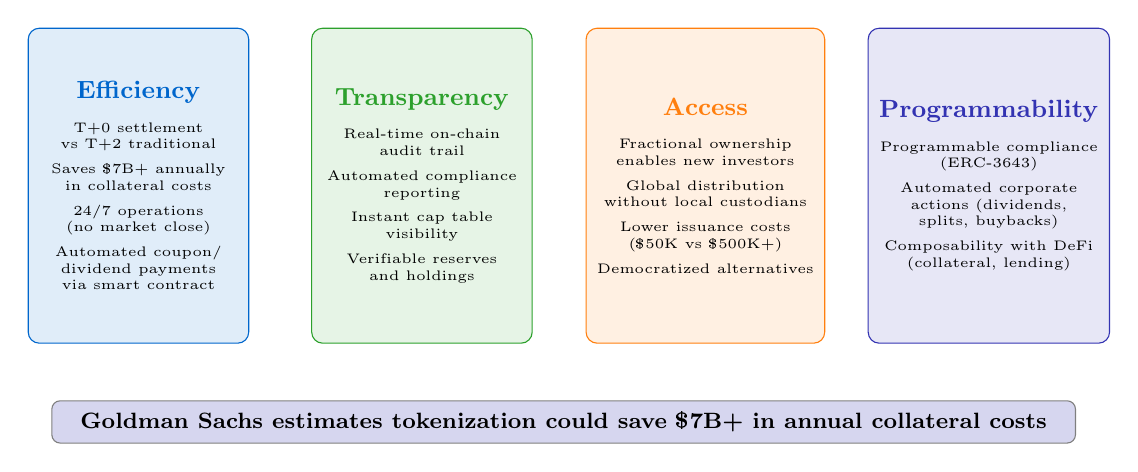
\begin{tikzpicture}[
  rwapillar/.style={draw,rounded corners=4pt,minimum width=2.8cm,minimum height=4.0cm,
    align=center,font=\tiny,inner sep=4pt}
]
  % Pillar 1: Efficiency
  \node[rwapillar,fill=mlblue!12,draw=mlblue] (pil1) at (0,0) {
    {\color{mlblue}\small\textbf{Efficiency}}\\[6pt]
    T+0 settlement\\vs T+2 traditional\\[3pt]
    Saves \$7B+ annually\\in collateral costs\\[3pt]
    24/7 operations\\(no market close)\\[3pt]
    Automated coupon/\\dividend payments\\via smart contract};
  % Pillar 2: Transparency
  \node[rwapillar,fill=mlgreen!12,draw=mlgreen] (pil2) at (3.6,0) {
    {\color{mlgreen}\small\textbf{Transparency}}\\[6pt]
    Real-time on-chain\\audit trail\\[3pt]
    Automated compliance\\reporting\\[3pt]
    Instant cap table\\visibility\\[3pt]
    Verifiable reserves\\and holdings};
  % Pillar 3: Access
  \node[rwapillar,fill=mlorange!12,draw=mlorange] (pil3) at (7.2,0) {
    {\color{mlorange}\small\textbf{Access}}\\[6pt]
    Fractional ownership\\enables new investors\\[3pt]
    Global distribution\\without local custodians\\[3pt]
    Lower issuance costs\\(\$50K vs \$500K+)\\[3pt]
    Democratized alternatives};
  % Pillar 4: Programmability
  \node[rwapillar,fill=mlpurple!12,draw=mlpurple] (pil4) at (10.8,0) {
    {\color{mlpurple}\small\textbf{Programmability}}\\[6pt]
    Programmable compliance\\(ERC-3643)\\[3pt]
    Automated corporate\\actions (dividends,\\splits, buybacks)\\[3pt]
    Composability with DeFi\\(collateral, lending)};
  % Foundation bar
  \node[draw=mlgray,fill=mllavender4,rounded corners=3pt,minimum width=13.0cm,
    font=\footnotesize\bfseries,inner sep=4pt,align=center] at (5.4,-3.0)
    {Goldman Sachs estimates tokenization could save \$7B+ in annual collateral costs};
\end{tikzpicture}
\bottomnote{The institutional case for tokenization is fundamentally about efficiency -- Goldman Sachs estimates tokenization could save \$7B+ in annual collateral costs}
\end{frame}

% Frame 46: Private Credit On-Chain
\begin{frame}{Private Credit On-Chain}
\begin{columns}[T]
\column{0.50\textwidth}
\vspace{2mm}
\footnotesize
\begin{block}{On-Chain Credit Protocols}
\begin{itemize}
  \item \textbf{Goldfinch:} emerging market lending (India, Kenya, SE Asia), \$100M+ originated, borrowers are fintech companies
  \item \textbf{Credix:} Latin American credit markets, trade finance and consumer lending
  \item \textbf{Clearpool:} institutional permissioned lending pools
  \item \textbf{TrueFi:} uncollateralized lending to vetted institutions
  \item Total on-chain private credit: \$500M+ active, \$4B+ cumulative
  \item Default rates: historically 2--5\% (similar to traditional private credit)
\end{itemize}
\end{block}

\column{0.48\textwidth}
\vspace{2mm}
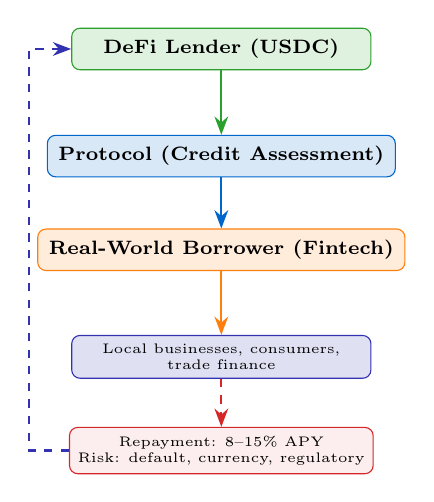
\begin{tikzpicture}[scale=0.85]
  % DeFi lender
  \node[draw=mlgreen,fill=mlgreen!15,rounded corners=3pt,minimum width=3.8cm,
    font=\scriptsize\bfseries,align=center,inner sep=4pt] (dlender) at (0,2.8)
    {DeFi Lender (USDC)};
  % Protocol
  \node[draw=mlblue,fill=mlblue!15,rounded corners=3pt,minimum width=3.8cm,
    font=\scriptsize\bfseries,align=center,inner sep=4pt] (proto) at (0,1.2)
    {Protocol (Credit Assessment)};
  % Borrower
  \node[draw=mlorange,fill=mlorange!15,rounded corners=3pt,minimum width=3.8cm,
    font=\scriptsize\bfseries,align=center,inner sep=4pt] (borrow) at (0,-0.2)
    {Real-World Borrower (Fintech)};
  % End borrowers
  \node[draw=mlpurple,fill=mlpurple!15,rounded corners=3pt,minimum width=3.8cm,
    font=\tiny,align=center,inner sep=3pt] (endborrow) at (0,-1.8)
    {Local businesses, consumers,\\trade finance};
  % Repayment
  \node[draw=mlred,fill=mlred!8,rounded corners=3pt,minimum width=3.8cm,
    font=\tiny,align=center,inner sep=3pt] (repay2) at (0,-3.2)
    {Repayment: 8--15\% APY\\Risk: default, currency, regulatory};
  % Arrows
  \draw[-{Stealth},thick,mlgreen] (dlender) -- (proto);
  \draw[-{Stealth},thick,mlblue] (proto) -- (borrow);
  \draw[-{Stealth},thick,mlorange] (borrow) -- (endborrow);
  \draw[-{Stealth},thick,dashed,mlred] (endborrow) -- (repay2);
  \draw[-{Stealth},thick,dashed,mlpurple] (repay2.west) -- ++(-0.6,0) |- (dlender.west);
\end{tikzpicture}
\end{columns}
\bottomnote{On-chain private credit brings DeFi yields to real-economy lending -- but carries real credit risk, as 2022 defaults demonstrated}
\end{frame}

% Frame 47: Section 4 Summary
\begin{frame}{Section 4 Summary: Real Estate \& Bond Tokenization}
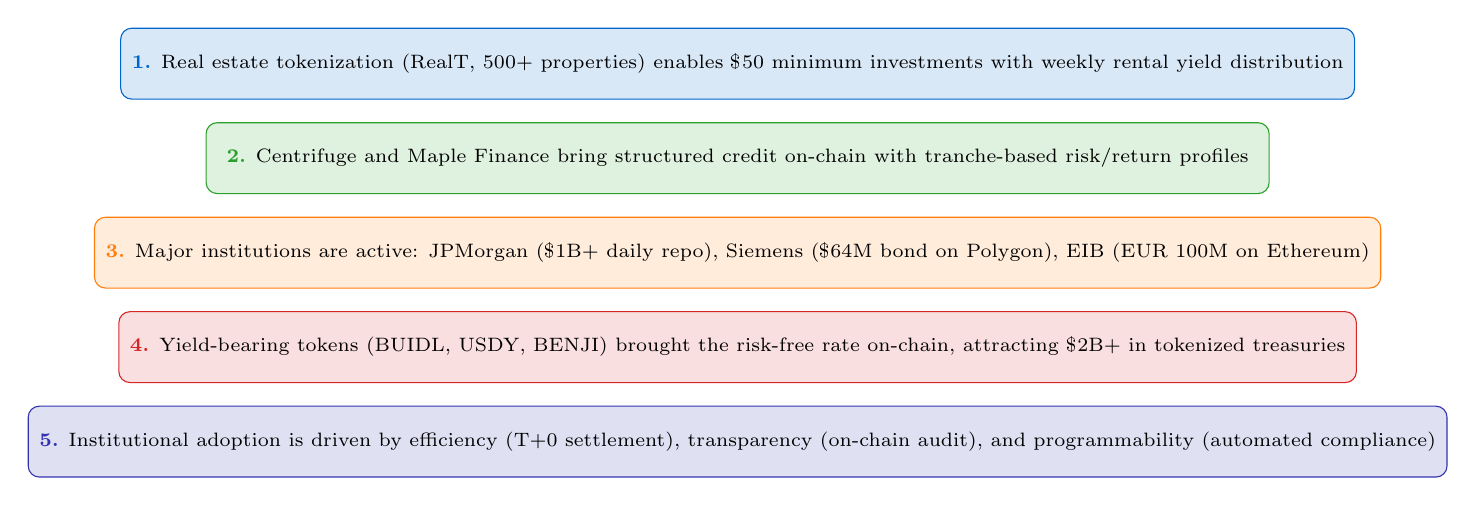
\begin{tikzpicture}[
  rwasummary/.style={draw,rounded corners=4pt,minimum width=13.5cm,minimum height=0.9cm,
    align=center,font=\scriptsize,inner sep=4pt}
]
  \node[rwasummary,fill=mlblue!15,draw=mlblue] at (6.5,2.0) {
    {\color{mlblue}\textbf{1.}} Real estate tokenization (RealT, 500+ properties) enables \$50 minimum investments with weekly rental yield distribution};
  \node[rwasummary,fill=mlgreen!15,draw=mlgreen] at (6.5,0.8) {
    {\color{mlgreen}\textbf{2.}} Centrifuge and Maple Finance bring structured credit on-chain with tranche-based risk/return profiles};
  \node[rwasummary,fill=mlorange!15,draw=mlorange] at (6.5,-0.4) {
    {\color{mlorange}\textbf{3.}} Major institutions are active: JPMorgan (\$1B+ daily repo), Siemens (\$64M bond on Polygon), EIB (EUR 100M on Ethereum)};
  \node[rwasummary,fill=mlred!15,draw=mlred] at (6.5,-1.6) {
    {\color{mlred}\textbf{4.}} Yield-bearing tokens (BUIDL, USDY, BENJI) brought the risk-free rate on-chain, attracting \$2B+ in tokenized treasuries};
  \node[rwasummary,fill=mlpurple!15,draw=mlpurple] at (6.5,-2.8) {
    {\color{mlpurple}\textbf{5.}} Institutional adoption is driven by efficiency (T+0 settlement), transparency (on-chain audit), and programmability (automated compliance)};
\end{tikzpicture}
\bottomnote{Section 4 complete | Next: Section 5 -- RWA Ecosystem \& Future}
\end{frame}

%% ============================================================
%% SECTION 5: RWA ECOSYSTEM & FUTURE
%% ============================================================
\section{RWA Ecosystem \& Future}

% Frame 48: Section 5 Divider
\begin{frame}{}
\begin{beamercolorbox}[sep=12pt,center,rounded=true,shadow=true]{palette quaternary}
  {\Large\bfseries Section 5: RWA Ecosystem \& Future}\\[6pt]
  {\normalsize Market projections, regulatory landscape, interoperability, and the future of tokenized finance}
\end{beamercolorbox}
\vspace{4mm}
\begin{columns}[T]
\column{0.5\textwidth}
\begin{block}{What You Will Learn}
\footnotesize
\begin{itemize}
  \item RWA market size projections (\$10--16T by 2030)
  \item BlackRock BUIDL and Ondo Finance as category leaders
  \item MakerDAO's RWA pivot and DeFi-TradFi convergence
  \item Regulatory challenges and the path to mainstream adoption
\end{itemize}
\end{block}
\column{0.5\textwidth}
\begin{block}{Frames in This Section}
\footnotesize
\begin{itemize}
  \item Frame 49: RWA Market Size Projections
  \item Frame 50: BlackRock BUIDL Fund
  \item Frame 51: Ondo Finance
  \item Frame 52: MakerDAO's RWA Pivot
  \item Frame 53: Regulatory Challenges
  \item Frame 54: TradFi-DeFi Convergence
  \item Frame 55: Key Takeaways and Course Summary
\end{itemize}
\end{block}
\end{columns}
\bottomnote{Section 5 covers the RWA ecosystem, major players, market projections, and the path forward for tokenized finance}
\end{frame}

% Frame 49: RWA Market Size Projections
\begin{frame}{RWA Market Size Projections}
\begin{columns}[T]
\column{0.50\textwidth}
\vspace{-2mm}
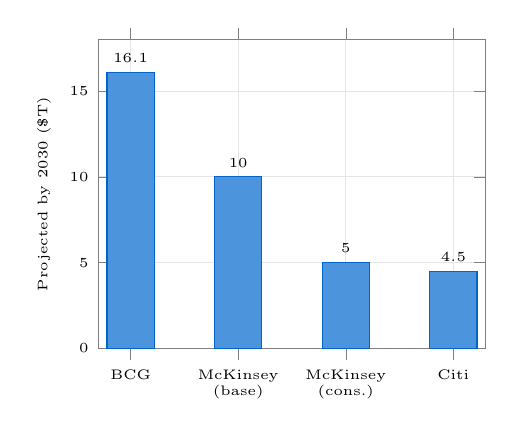
\begin{tikzpicture}
\begin{axis}[
  ybar,
  width=6.5cm, height=5.5cm,
  bar width=0.6cm,
  xlabel={},
  ylabel={Projected by 2030 (\$T)},
  ylabel style={font=\tiny},
  xlabel style={font=\tiny},
  ymin=0, ymax=18,
  xtick=data,
  symbolic x coords={BCG, McKinsey\\(base), McKinsey\\(cons.), Citi},
  xticklabel style={font=\tiny,align=center},
  yticklabel style={font=\tiny},
  nodes near coords,
  every node near coord/.append style={font=\tiny\bfseries},
  grid=major,
  grid style={gray!20},
  axis line style={mlgray},
]
\addplot[fill=mlblue!70,draw=mlblue] coordinates {
  (BCG, 16.1)
  (McKinsey\\(base), 10)
  (McKinsey\\(cons.), 5)
  (Citi, 4.5)
};
\end{axis}
\end{tikzpicture}

\vspace{1mm}
\centering\tiny Current (2024/2025): \textasciitilde\$5B tokenized (excl.\ stablecoins)\\
Growth multiple: 1{,}000--3{,}000x in 5--6 years

\column{0.48\textwidth}
\vspace{2mm}
\begin{block}{Breakdown by Asset Class (2030 Projected)}
\footnotesize
\begin{itemize}
  \item \textbf{Tokenized funds \& bonds:} \$5T (40\%)
  \item \textbf{Tokenized real estate:} \$3T (25\%)
  \item \textbf{Tokenized trade finance:} \$2T (15\%)
  \item \textbf{Tokenized securities:} \$1T (8\%)
  \item \textbf{Other} (art, IP, carbon, commodities): \$1.5T (12\%)
\end{itemize}
\end{block}
\vspace{2mm}
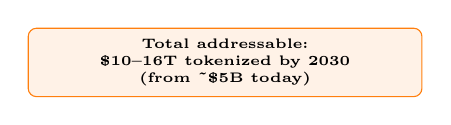
\begin{tikzpicture}
  \node[draw=mlorange,fill=mlorange!10,rounded corners=3pt,minimum width=5.0cm,
    align=center,font=\tiny\bfseries,inner sep=4pt] {
    Total addressable:\\
    \$10--16T tokenized by 2030\\
    (from \textasciitilde\$5B today)};
\end{tikzpicture}
\end{columns}
\bottomnote{Even conservative estimates project 1000x growth -- the question is not if tokenization will happen, but how fast regulation and infrastructure enable it}
\end{frame}

% Frame 50: BlackRock BUIDL Fund
\begin{frame}{BlackRock BUIDL Fund}
\begin{columns}[T]
\column{0.50\textwidth}
\vspace{2mm}
\footnotesize
\begin{block}{BUIDL Details}
\begin{itemize}
  \item \textbf{Product:} BlackRock USD Institutional Digital Liquidity Fund
  \item \textbf{Asset:} Short-term US Treasury bills
  \item \textbf{Blockchain:} Ethereum (primary), expanding to Avalanche, Polygon, Optimism, Arbitrum via Securitize
  \item \textbf{AUM:} \$500M+ (largest tokenized fund)
  \item \textbf{Minimum:} \$5M (institutional)
  \item \textbf{Yield:} \textasciitilde5\% APY (passes through T-bill yield)
  \item \textbf{Token:} daily NAV rebase, instant transfers
  \item \textbf{Partners:} Securitize (platform), BNY Mellon (custody), PwC (audit)
  \item \textbf{Significance:} BlackRock = \$10T AUM, world's largest asset manager
\end{itemize}
\end{block}

\column{0.48\textwidth}
\vspace{2mm}
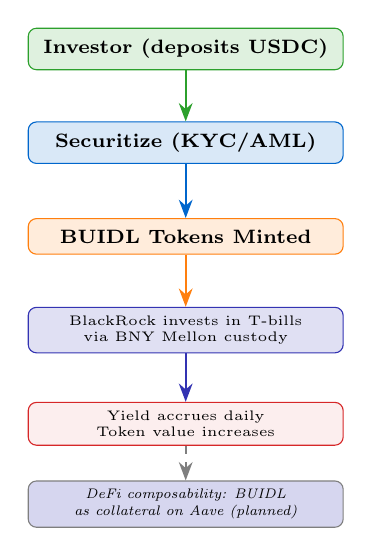
\begin{tikzpicture}[scale=0.85]
  % Investor
  \node[draw=mlgreen,fill=mlgreen!15,rounded corners=3pt,minimum width=4.0cm,
    font=\scriptsize\bfseries,align=center,inner sep=4pt] (inv) at (0,3.0)
    {Investor (deposits USDC)};
  % Securitize KYC
  \node[draw=mlblue,fill=mlblue!15,rounded corners=3pt,minimum width=4.0cm,
    font=\scriptsize\bfseries,align=center,inner sep=4pt] (sec) at (0,1.6)
    {Securitize (KYC/AML)};
  % BUIDL tokens
  \node[draw=mlorange,fill=mlorange!15,rounded corners=3pt,minimum width=4.0cm,
    font=\scriptsize\bfseries,align=center,inner sep=4pt] (buidl) at (0,0.2)
    {BUIDL Tokens Minted};
  % BlackRock invests
  \node[draw=mlpurple,fill=mlpurple!15,rounded corners=3pt,minimum width=4.0cm,
    font=\tiny,align=center,inner sep=3pt] (br) at (0,-1.2)
    {BlackRock invests in T-bills\\via BNY Mellon custody};
  % Yield
  \node[draw=mlred,fill=mlred!8,rounded corners=3pt,minimum width=4.0cm,
    font=\tiny,align=center,inner sep=3pt] (yld) at (0,-2.6)
    {Yield accrues daily\\Token value increases};
  % DeFi
  \node[draw=mlgray,fill=mllavender4,rounded corners=3pt,minimum width=4.0cm,
    font=\tiny\itshape,align=center,inner sep=3pt] (defi) at (0,-3.8)
    {DeFi composability: BUIDL\\as collateral on Aave (planned)};
  % Arrows
  \draw[-{Stealth},thick,mlgreen] (inv) -- (sec);
  \draw[-{Stealth},thick,mlblue] (sec) -- (buidl);
  \draw[-{Stealth},thick,mlorange] (buidl) -- (br);
  \draw[-{Stealth},thick,mlpurple] (br) -- (yld);
  \draw[-{Stealth},thick,dashed,mlgray] (yld) -- (defi);
\end{tikzpicture}
\end{columns}
\bottomnote{When the world's largest asset manager (\$10T AUM) launches a tokenized fund on Ethereum, it signals institutional conviction that blockchain is the future of finance}
\end{frame}

% Frame 51: Ondo Finance
\begin{frame}{Ondo Finance}
\begin{columns}[T]
\column{0.50\textwidth}
\vspace{2mm}
\footnotesize
\begin{block}{Ondo Products}
\begin{itemize}
  \item \textbf{USDY:} yield-bearing stablecoin backed by T-bills and bank deposits, 5.2\% APY, \$300M+
  \item \textbf{OUSG:} tokenized short-term US government bonds
  \item Multi-chain: Ethereum, Solana, Mantle, Sui, Aptos
  \item \textbf{Ondo Global Markets:} planned tokenized equities and ETFs
  \item \textbf{Flux Finance:} DeFi lending protocol for tokenized treasuries
  \item Investment: backed by Pantera, Coinbase Ventures, Founders Fund
  \item Regulatory approach: Reg D/Reg S exemptions, KYC required
\end{itemize}
\end{block}

\column{0.48\textwidth}
\vspace{2mm}
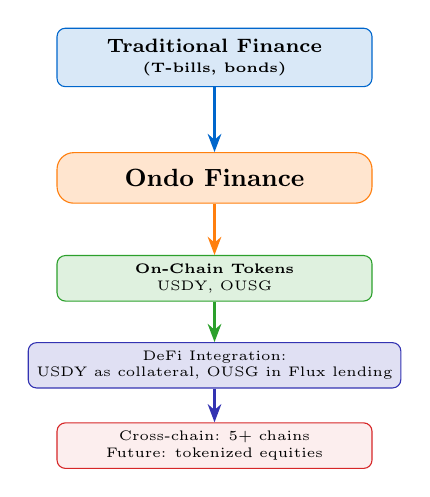
\begin{tikzpicture}[scale=0.85]
  % TradFi
  \node[draw=mlblue,fill=mlblue!15,rounded corners=3pt,minimum width=4.0cm,
    font=\scriptsize\bfseries,align=center,inner sep=4pt] (tradfi) at (0,2.8)
    {Traditional Finance\\[-1pt]\tiny (T-bills, bonds)};
  % Ondo
  \node[draw=mlorange,fill=mlorange!20,rounded corners=6pt,minimum width=4.0cm,
    font=\small\bfseries,align=center,inner sep=6pt] (ondo) at (0,1.0)
    {Ondo Finance};
  % Tokens
  \node[draw=mlgreen,fill=mlgreen!15,rounded corners=3pt,minimum width=4.0cm,
    font=\tiny,align=center,inner sep=3pt] (tokens) at (0,-0.5)
    {\textbf{On-Chain Tokens}\\USDY, OUSG};
  % DeFi integration
  \node[draw=mlpurple,fill=mlpurple!15,rounded corners=3pt,minimum width=4.0cm,
    font=\tiny,align=center,inner sep=3pt] (defiint) at (0,-1.8)
    {DeFi Integration:\\USDY as collateral, OUSG in Flux lending};
  % Cross-chain
  \node[draw=mlred,fill=mlred!8,rounded corners=3pt,minimum width=4.0cm,
    font=\tiny,align=center,inner sep=3pt] (cross) at (0,-3.0)
    {Cross-chain: 5+ chains\\Future: tokenized equities};
  % Arrows
  \draw[-{Stealth},thick,mlblue] (tradfi) -- (ondo);
  \draw[-{Stealth},thick,mlorange] (ondo) -- (tokens);
  \draw[-{Stealth},thick,mlgreen] (tokens) -- (defiint);
  \draw[-{Stealth},thick,mlpurple] (defiint) -- (cross);
\end{tikzpicture}
\end{columns}
\bottomnote{Ondo is the bridge between TradFi yield and DeFi composability -- its multi-chain approach makes Treasury yields accessible across the crypto ecosystem}
\end{frame}

% Frame 52: MakerDAO's RWA Pivot
\begin{frame}{MakerDAO's RWA Pivot}
\begin{columns}[T]
\column{0.50\textwidth}
\vspace{2mm}
\footnotesize
\begin{block}{MakerDAO (now Sky) RWA Journey}
\begin{itemize}
  \item \textbf{2020:} First RWA collateral (Centrifuge assets)
  \item \textbf{2022:} \$500M allocated to US Treasuries (via Monetalis Clydesdale)
  \item \textbf{2023:} RWA allocation reaches \$2B+ (largest DeFi-to-TradFi bridge)
  \item \textbf{2024:} RWA represents 40\%+ of DAI backing
  \item Collateral types:
    \begin{itemize}\tiny
      \item US Treasury bills (\$1.5B+ via BlockTower, Monetalis)
      \item Centrifuge pools (trade finance, real estate)
      \item Coinbase USDC institutional custody
    \end{itemize}
  \item Revenue: RWA vaults generate 60\%+ of MakerDAO revenue
  \item Controversy: centralization concerns -- DAI now depends heavily on TradFi assets
\end{itemize}
\end{block}

\column{0.48\textwidth}
\vspace{2mm}
\centering
{\scriptsize\textbf{DAI Backing Composition}}
\vspace{2mm}
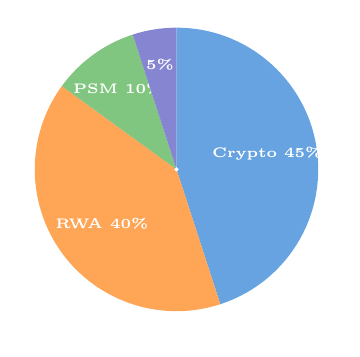
\begin{tikzpicture}[scale=0.9]
  % Pie chart using manual arcs
  % Crypto 45% = 162 degrees
  \fill[mlblue!60] (0,0) -- (90:2.0) arc (90:-72:2.0) -- cycle;
  \node[font=\tiny\bfseries,text=white] at (10:1.3) {Crypto 45\%};
  % RWA 40% = 144 degrees
  \fill[mlorange!70] (0,0) -- (-72:2.0) arc (-72:-216:2.0) -- cycle;
  \node[font=\tiny\bfseries,text=white] at (-144:1.3) {RWA 40\%};
  % PSM 10% = 36 degrees
  \fill[mlgreen!60] (0,0) -- (-216:2.0) arc (-216:-252:2.0) -- cycle;
  \node[font=\tiny\bfseries,text=white] at (-234:1.4) {PSM 10\%};
  % Other 5% = 18 degrees
  \fill[mlpurple!60] (0,0) -- (-252:2.0) arc (-252:-270:2.0) -- cycle;
  \node[font=\tiny\bfseries,text=white] at (-261:1.5) {5\%};
  % Center label
  \draw[white,thick] (0,0) circle (0.01);
\end{tikzpicture}

\vspace{2mm}
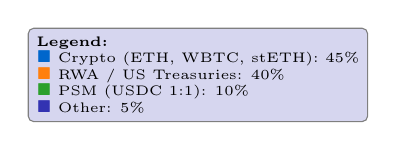
\begin{tikzpicture}
  \node[draw=mlgray,fill=mllavender4,rounded corners=2pt,font=\tiny,align=left,inner sep=3pt] {
    \textbf{Legend:}\\
    {\color{mlblue}$\blacksquare$} Crypto (ETH, WBTC, stETH): 45\%\\
    {\color{mlorange}$\blacksquare$} RWA / US Treasuries: 40\%\\
    {\color{mlgreen}$\blacksquare$} PSM (USDC 1:1): 10\%\\
    {\color{mlpurple}$\blacksquare$} Other: 5\%
  };
\end{tikzpicture}
\end{columns}
\bottomnote{MakerDAO's RWA pivot is the most significant DeFi-TradFi convergence event -- \$2B+ in Treasury bills backing a decentralized stablecoin}
\end{frame}

% Frame 53: Regulatory Challenges & Legal Gaps
\begin{frame}{Regulatory Challenges \& Legal Gaps}
\vspace{-2mm}
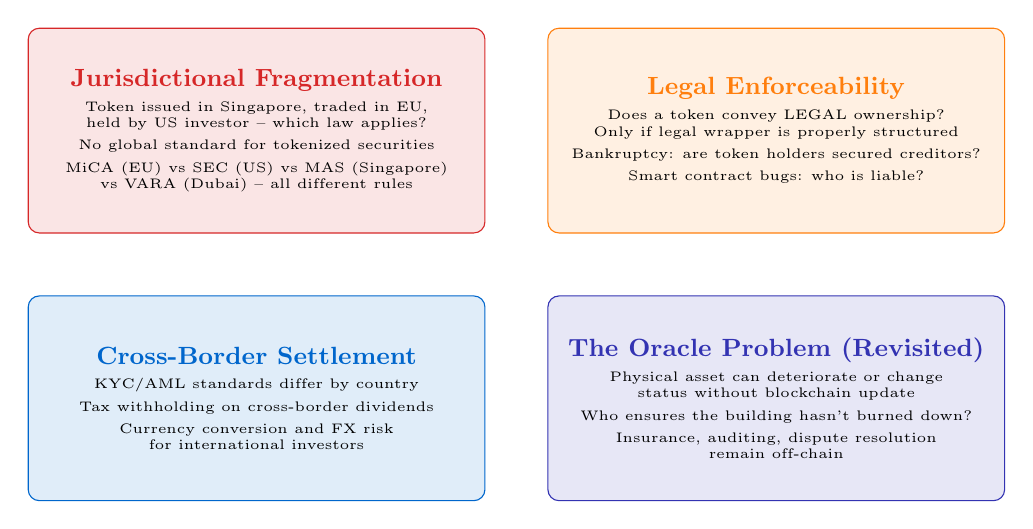
\begin{tikzpicture}[
  rwachallenge/.style={draw,rounded corners=4pt,minimum width=5.8cm,minimum height=2.6cm,
    align=center,font=\tiny,inner sep=4pt}
]
  % Challenge 1: Jurisdictional Fragmentation
  \node[rwachallenge,fill=mlred!12,draw=mlred] (ch1) at (3.2,1.5) {
    {\color{mlred}\small\textbf{Jurisdictional Fragmentation}}\\[3pt]
    Token issued in Singapore, traded in EU,\\held by US investor -- which law applies?\\[2pt]
    No global standard for tokenized securities\\[2pt]
    MiCA (EU) vs SEC (US) vs MAS (Singapore)\\vs VARA (Dubai) -- all different rules};
  % Challenge 2: Legal Enforceability
  \node[rwachallenge,fill=mlorange!12,draw=mlorange] (ch2) at (9.8,1.5) {
    {\color{mlorange}\small\textbf{Legal Enforceability}}\\[3pt]
    Does a token convey LEGAL ownership?\\Only if legal wrapper is properly structured\\[2pt]
    Bankruptcy: are token holders secured creditors?\\[2pt]
    Smart contract bugs: who is liable?};
  % Challenge 3: Cross-Border Settlement
  \node[rwachallenge,fill=mlblue!12,draw=mlblue] (ch3) at (3.2,-1.9) {
    {\color{mlblue}\small\textbf{Cross-Border Settlement}}\\[3pt]
    KYC/AML standards differ by country\\[2pt]
    Tax withholding on cross-border dividends\\[2pt]
    Currency conversion and FX risk\\for international investors};
  % Challenge 4: The Oracle Problem
  \node[rwachallenge,fill=mlpurple!12,draw=mlpurple] (ch4) at (9.8,-1.9) {
    {\color{mlpurple}\small\textbf{The Oracle Problem (Revisited)}}\\[3pt]
    Physical asset can deteriorate or change\\status without blockchain update\\[2pt]
    Who ensures the building hasn't burned down?\\[2pt]
    Insurance, auditing, dispute resolution\\remain off-chain};
\end{tikzpicture}
\bottomnote{Regulation is the biggest barrier to RWA growth -- technology is ready, legal frameworks are not, and fragmentation across jurisdictions creates friction}
\end{frame}

% Frame 54: TradFi-DeFi Convergence
\begin{frame}{TradFi-DeFi Convergence}
\vspace{-2mm}
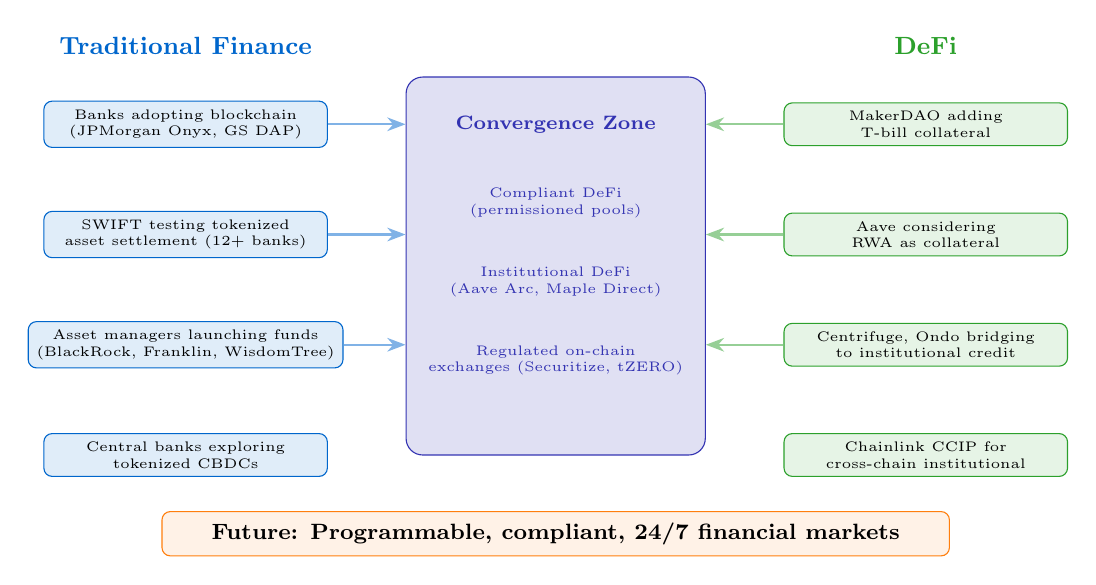
\begin{tikzpicture}[
  rwaconv/.style={draw,rounded corners=3pt,minimum width=3.6cm,font=\tiny,
    align=center,inner sep=3pt}
]
  % Left: TradFi
  \node[font=\small\bfseries,text=mlblue] at (1.8,2.8) {Traditional Finance};
  \node[rwaconv,fill=mlblue!12,draw=mlblue] (tf1) at (1.8,1.8) {
    Banks adopting blockchain\\(JPMorgan Onyx, GS DAP)};
  \node[rwaconv,fill=mlblue!12,draw=mlblue] (tf2) at (1.8,0.4) {
    SWIFT testing tokenized\\asset settlement (12+ banks)};
  \node[rwaconv,fill=mlblue!12,draw=mlblue] (tf3) at (1.8,-1.0) {
    Asset managers launching funds\\(BlackRock, Franklin, WisdomTree)};
  \node[rwaconv,fill=mlblue!12,draw=mlblue] (tf4) at (1.8,-2.4) {
    Central banks exploring\\tokenized CBDCs};

  % Right: DeFi
  \node[font=\small\bfseries,text=mlgreen] at (11.2,2.8) {DeFi};
  \node[rwaconv,fill=mlgreen!12,draw=mlgreen] (df1) at (11.2,1.8) {
    MakerDAO adding\\T-bill collateral};
  \node[rwaconv,fill=mlgreen!12,draw=mlgreen] (df2) at (11.2,0.4) {
    Aave considering\\RWA as collateral};
  \node[rwaconv,fill=mlgreen!12,draw=mlgreen] (df3) at (11.2,-1.0) {
    Centrifuge, Ondo bridging\\to institutional credit};
  \node[rwaconv,fill=mlgreen!12,draw=mlgreen] (df4) at (11.2,-2.4) {
    Chainlink CCIP for\\cross-chain institutional};

  % Center: Convergence zone
  \node[draw=mlpurple,fill=mlpurple!15,rounded corners=6pt,minimum width=3.8cm,
    minimum height=4.8cm,inner sep=4pt] (center) at (6.5,0.0) {};
  \node[font=\scriptsize\bfseries,text=mlpurple] at (6.5,1.8) {Convergence Zone};
  \node[font=\tiny,align=center,text=mlpurple] at (6.5,0.8) {Compliant DeFi\\(permissioned pools)};
  \node[font=\tiny,align=center,text=mlpurple] at (6.5,-0.2) {Institutional DeFi\\(Aave Arc, Maple Direct)};
  \node[font=\tiny,align=center,text=mlpurple] at (6.5,-1.2) {Regulated on-chain\\exchanges (Securitize, tZERO)};

  % Arrows from TradFi to center
  \draw[-{Stealth},thick,mlblue!50] (tf1.east) -- (center.west |- tf1);
  \draw[-{Stealth},thick,mlblue!50] (tf2.east) -- (center.west |- tf2);
  \draw[-{Stealth},thick,mlblue!50] (tf3.east) -- (center.west |- tf3);
  % Arrows from DeFi to center
  \draw[-{Stealth},thick,mlgreen!50] (df1.west) -- (center.east |- df1);
  \draw[-{Stealth},thick,mlgreen!50] (df2.west) -- (center.east |- df2);
  \draw[-{Stealth},thick,mlgreen!50] (df3.west) -- (center.east |- df3);

  % Future vision
  \node[draw=mlorange,fill=mlorange!10,rounded corners=3pt,minimum width=10.0cm,
    font=\footnotesize\bfseries,inner sep=4pt,align=center] at (6.5,-3.4)
    {Future: Programmable, compliant, 24/7 financial markets};
\end{tikzpicture}
\bottomnote{The convergence is bidirectional: TradFi is coming to blockchain AND DeFi is becoming regulated -- the middle ground is ``institutional DeFi''}
\end{frame}

% Frame 55: Key Takeaways and Course Summary
\begin{frame}{Key Takeaways and Course Summary}
\vspace{-2mm}
\begin{tikzpicture}[
  rwatakeaway/.style={draw,rounded corners=4pt,minimum width=13.5cm,minimum height=0.9cm,
    align=center,font=\scriptsize,inner sep=4pt}
]
  \node[rwatakeaway,fill=mlblue!15,draw=mlblue] at (6.5,2.2) {
    {\color{mlblue}\textbf{1. Tokenization Fundamentals}} -- tokenization digitizes asset ownership via blockchain + legal wrappers; ERC-3643 enables compliant security tokens};
  \node[rwatakeaway,fill=mlpurple!15,draw=mlpurple] at (6.5,1.0) {
    {\color{mlpurple}\textbf{2. Stablecoins}} -- \$150B+ market, fiat-backed dominates; Terra/Luna proved algorithmic models are fatally flawed; MiCA sets regulatory template};
  \node[rwatakeaway,fill=mlgreen!15,draw=mlgreen] at (6.5,-0.2) {
    {\color{mlgreen}\textbf{3. Security Tokens \& Compliance}} -- Howey test determines classification; on-chain KYC/AML via identity registries; SPVs bridge legal and digital worlds};
  \node[rwatakeaway,fill=mlorange!15,draw=mlorange] at (6.5,-1.4) {
    {\color{mlorange}\textbf{4. Real Estate \& Bonds}} -- RealT (500+ properties), JPMorgan (\$1B+ daily), BlackRock BUIDL (\$500M+); yield-bearing tokens bring risk-free rate on-chain};
  \node[rwatakeaway,fill=mlred!15,draw=mlred] at (6.5,-2.6) {
    {\color{mlred}\textbf{5. RWA Future}} -- \$10--16T projected by 2030; TradFi and DeFi converging; regulation is the biggest barrier; institutional conviction is accelerating};
  % Teal teaser bar
  \node[fill=teal!80,text=white,rounded corners=3pt,minimum width=13.5cm,
    font=\footnotesize\bfseries,inner sep=5pt,align=center] at (6.5,-3.8)
    {Next: Advanced topics in DeFi-TradFi integration, CBDC design, and cross-chain institutional infrastructure};
\end{tikzpicture}
\bottomnote{Course complete | 5 sections, 55 frames | From tokenization fundamentals to the future of real-world assets on-chain}
\end{frame}

\end{document}
